\documentclass[11pt]{article}

%\pagestyle{headings}

\textwidth=440pt
\hoffset=-0.6truein

\usepackage{amsmath}
\usepackage{amsfonts}
\usepackage{amssymb}
\usepackage{dsfont}
\usepackage{pifont}
\usepackage{booktabs}
\usepackage{tabularx}
\usepackage{siunitx}
%\usepackage{bbold}
\usepackage{graphicx}
\usepackage{epstopdf}
\usepackage{epsfig}
%\usepackage{bibunits}
%\usepackage{theorem}
\usepackage[framed]{ntheorem}
\usepackage{framed}
%\usepackage{showlabels}
\usepackage{makeidx}
\usepackage{simplewick}
%\usepackage{tikz-feynman}
\usepackage{hyperref}
\usepackage{placeins}
\usepackage[font=small,labelfont=bf]{caption}
%\tikzfeynmanset{compat=1.0.0}

% barn deprecated by siunitx
\DeclareSIUnit{\barn}{b}

% General global commands
\newcommand{\cov}{C}
\newcommand{\posterior}[1]{\tilde{#1}}
\newcommand{\real}{\mathbb{R}}

% General inverse Problems
% map operators
\newcommand{\fwdmapop}{G}
\newcommand{\obsop}{O}
\newcommand{\fwdobsop}{\mathcal{\fwdmapop}}
% model space
\newcommand{\nmodel}{N_{\rm model}}
\newcommand{\modelspace}{X}
\newcommand{\modelvec}{u}
\newcommand{\modelpriorcent}{\modelvec_0}
\newcommand{\modelpriorcov}{\cov_M}
\newcommand{\modelpostcent}{\posterior{\modelvec}}
\newcommand{\modelpostcov}{\posterior{\cov}_M}
% observable space
\newcommand{\ndata}{N_{\rm data}}
\newcommand{\obs}{y}
\newcommand{\obspriorcent}{\obs_0}
\newcommand{\obspriorcov}{\cov_{D}}
\newcommand{\obsnoise}{\eta}
\newcommand{\obspostcent}{\posterior{\obs}}
\newcommand{\obspostcov}{\posterior{\cov}_D}
% linear map
\newcommand{\linmap}{\fwdobsop}
\newcommand{\vander}{\mathcal{X}}
\newcommand{\nlaw}{N_{\rm law}}

% NNPDF data/model
\newcommand{\law}{f}
\newcommand{\pseudodat}{\mu}
\newcommand{\noise}{\epsilon}
\newcommand{\repind}{(k)}
\newcommand{\modelvecrep}{\modelvec_*^{\repind}}
% likelihood
\newcommand{\likelihood}{\mathcal{L}}
\newcommand{\repchis}{{\chi^2}^{\repind}}

% closure fitting
\newcommand{\lawmodel}{w}
\newcommand{\utrue}{u_\mathrm{true}}
\newcommand{\uest}{u_\mathrm{est}}

% closure estimators
\newcommand{\testset}[1]{ {{#1}^{\prime}} }
\newcommand{\emodel}[1]{ \mathbf{E}_{\{ \modelvec_* \}} \left[ #1 \right] }
\newcommand{\eout}{\mathcal{E}^{\rm out}}

\newcommand{\nfits}{N_{\rm fits}}
\newcommand{\nreps}{N_{\rm replicas}}

\newcommand{\bias}{{\rm bias}}
\newcommand{\var}{{\rm variance}}
\newcommand{\covrep}{\testset{\cov}^{(\rm replica)}}
\newcommand{\covcent}{\testset{\cov}^{(\rm central)}}
\newcommand{\biasvarratio}{\mathcal{R}_{bv}}

% quantile estimators
\newcommand{\xisigdat}[1]{\xi^{(\rm data)}_{#1 \sigma}}
\newcommand{\xisigdati}[1]{\xi^{(\rm data)}_{#1 {\sigma^i}}}
\newcommand{\modelstd}{\hat{\sigma}}
\newcommand{\erf}{{\rm erf}}

% abbreviations
\newcommand{\ie}{{\it i.e.}}
\newcommand{\eg}{{\it e.g.}}
\newcommand{\viz}{{\it viz.}}

% delta chi2 appendix
\newcommand{\ein}{\mathcal{E}^{\rm in}}
\newcommand{\deltachi}{\Delta_{\chi^2}}
\newcommand{\noisecross}{{\rm noise \, cross \, term}}

% -------------------%
% deprecated commands
% -------------------%
\newcommand{\vv}[1]{\mathbf{#1}}

\newcommand{\vecdiffreptwo}{\left( \vv{\model}^{\repind} - \vv{\levtwo}^{\repind}  \right)}
\newcommand{\vecdiffcentone}{\left( \erep{\vv{\model}} - \vv{\levone} \right)}

\newcommand{\coveig}{\sigma^{2}}
\newcommand{\diag}[1]{\hat{#1}}

\newcommand{\levelonediff}{\Delta}
\newcommand{\underlyingdiff}{u}
\newcommand{\repdiff}{v}

\newcommand{\shiftcross}{{\rm shift \, cross \, term}}
\newcommand{\deltaeps}{\Delta_{\epsilon}}
\newcommand{\kldiv}{D_{KL}}

\newcommand{\diffreptwo}{\left( \model^{\repind} - \levtwo^{\repind} \right)}
\newcommand{\diffcentone}{\left( \erep{\model} - \levone \right)}
\newcommand{\diffcentunder}{\left( \erep{\model} - \law \right)}
\newcommand{\diffcentrep}{\left( \erep{\model} - \model^{\repind}\right)}

\newcommand{\invcov}[1]{\cov^{-1}_{#1}}
\newcommand{\erep}[1]{\mathbf{E}_{\noise}\left[ #1 \right]}
\newcommand{\eshift}[1]{\mathbf{E}_{\shift}\left[ #1 \right]}

\newcommand{\model}{\fwdobsop}
\newcommand{\shift}{\obsnoise}
\newcommand{\invcovprime}{C_D^{\prime -1}}
\newcommand{\levone}{z}
\newcommand{\levtwo}{y}

\newcommand{\npoints}{N_{\rm points}}
\newcommand{\nfit}{\texttt{n3fit}}

\graphicspath{{./figures/}}

\title{Bayesian Approach to Inverse Problems: an Application to NNPDF Closure Testing}
\author[a]{Luigi Del Debbio} 
\author[a]{Tommaso Giani} 
\author[a]{Michael Wilson}
\affil[a]{Higgs Centre for Theoretical Physics, School of Physics and Astronomy,
Peter~Guthrie~Tait~Road, Edinburgh EH9 3 FD, United Kingdom.}


\makeindex

\begin{document}

\maketitle

\begin{abstract}
    We discuss the Bayesian approach to the solution of inverse problems and
    apply the formalism to analyse the closure tests performed by the NNPDF
    collaboration. Starting from a comparison with the approach that is
    currently used for the determination of parton distributions (PDFs) by the
    NNPDF collaboration, we discuss some analytical results that can be obtained
    for linear problems and use these results as a guidance for the more
    complicated non-linear problems. We show that, in the case of Gaussian
    distributions, the posterior probability density of the parametrized PDFs is
    fully determined by the results of the NNPDF fitting procedure. In the
    particular case that we consider, the fitting procedure and the Bayesian
    analysis yield exactly the same result. Building on the insight that we
    obtain from the analytical results, we introduce new estimators to assess
    the statistical faithfulness of the fit results in closure tests. These
    estimators are defined in data space, and can be studied analytically using
    the Bayesian formalism in a linear model in order to clarify their meaning.
    Finally we present numerical results from a number of closure tests
    performed with current NNPDF methodologies. These further tests allow us to
    validate the new methodology and provide a quantitative comparison of the
    new and old methodologies. As PDFs determinations move into precision
    territory, the need for a careful validation of the methodology becomes
    increasingly important: the error bar has become the focal point of
    contemporary PDFs determinations. In this perspective, theoretical
    assumptions and other sources of error are best formulated and analysed in
    the Bayesian framework, which provides an ideal language to address the
    precision and the accuracy of current fits. 

\end{abstract}

\section{Introduction}

In an NNPDF fit to experimental data, a set of replicas are fitted to pseudodata
which is generated according the experimental central values and uncertainties.
A successful fit is realised if the resulting replicas agree with the underlying
law within uncertainties. Since the underlying law is usually unknown we cannot
directly measure if this is the case.

We can, however, test the methodology in a fit to artificial data, which is
generated from theory predictions from an input PDF and check that we agree with
the input PDF within uncertainties. This is the basis of a closure test, which
has already been used to test to validity of previous iterations of the NNPDF
methodology. Here we aim to refine some of the pre-existing closure test
estimators and with the help of fast fitting methodology perform a more
extensive study of how faithful our uncertainties are.

When fitting experimental data we vary the parameters of a set of PDF replicas
at the initial scale such that the $\chi^2$ is minimised between the
corresponding theory predictions and a generated pseudodata replica. A set of
PDFs usually refers to a set of seperate continuous functions, one for each
flavour of PDF in a particular basis. In this specific study, fits performed
with \nfit\ parameterise the set of PDFs as a single neural network which takes
as input $x$ and $\ln x$ and returns 8 outputs, one for each flavour in the
fitting basis, multiplied by some preproccessing exponents. The output for a
single flavour $j$ is
\begin{equation}
    N(x, \ln x)_j * x^{1-\alpha_j} * (1-x)^{\beta_j},
\end{equation}
where each flavour has its own preproccessing exponents $\alpha$ and $\beta$
which are parameters which are varied in these fits. The pseudodata replica is
generated through Monte Carlo sampling according to the experimental
uncertainty, by applying a shift to the experimental central values. After
fitting many sets of PDF replicas (usually of order 100 sets), each set to an
independently generated pseudodata replica, we have an ensemble of PDF replicas
which is a sample of the probability distribution of the PDF given the data. The
aim of this methodology, is to propagate the various sources of uncertainty
involved with fitting PDFs into the functional PDF space. If we consider
experimental data which we assume to be multigaussian then the experimental
central values, $\levone$, are given by
\begin{equation}
    \levone_{i} = \law_i + \shift_i
\end{equation}
in other words, the experimental values have been shifted away from the true
values given by nature, $\law$, by some shift, $\shift$. The shift is drawn from
the multigaussian $\mathcal{N}(0, \cov)$ where $\cov$ is the experimental
covariance matrix. The fitted pseudodata is obtained by adding Monte Carlo
noise, $\noise^{\repind}$, on top of the experimental central values
\begin{equation}
    \levtwo^{\repind}_{i} = \law_i + \shift_i + \noise^{\repind}_{i},
\end{equation}
where the replica index $k$ refers to each replica having different noise drawn
independently from $\mathcal{N}(0, \cov)$. The $\chi^2$ which is minimised for
replica $k$ is then given by
\begin{equation}
    \repchis = \frac{1}{\ndata} \sum_{ij} \diffreptwo_i \invcov{ij} \diffreptwo_j,
\end{equation}
where $\model^{\repind}_i$ is the prediction for $i^{\rm th}$ datapoint, from
the $k^{\rm th}$ set of PDFs. After fitting many replicas, the quality of a fit
is often determined by considering the $\chi^2$ between the experimental central
values and the expectation value of the theory predictions
\begin{equation}\label{eq:centralchi2}
    \chi^2 = \frac{1}{\ndata} \sum_{ij} \diffcentone_i \invcov{ij} \diffcentone_j,
\end{equation}
where $\erep{\cdot}$ denotes the mean value across replicas, so $\erep{g}$ is
the mean of the theory predictions across replicas. This $\chi^2$ is a measure
of the difference between the expectation value of the prediction and the
experimental central values in units of the covariance.

In a fit to experimental data we are limited to this quantity because we don't
have knowledge of the underlying theory predictions of nature $\law$. In a
closure test we use a pre-existing PDF as an input to obtain $\law$ and then
generate both $\shift$ and $\noise$ from $\mathcal{N}(0, \cov)$, emulating the
different levels of data. The underlying theory predictions are referred to as
level zero data. We refer to the shifted central values as level one data, the
underlying law plus a level one shift. The pseudodata which a given replica fits
is then referred to as level two data.


\section{Inverse Problems}
\label{sec:inverse-problems}

The problem of determining PDFs from a set of experimental data falls under the
general category of {\em inverse problems}, \ie\ the problem of finding the
input to a given model knowing a set of observations, which are often finite and
noisy. In this section we are going to review the Bayesian formulation of
inverse problems. It is impossible to do justice to this vast subject here.
Instead we try to emphasise the aspects that are relevant for quantifying
uncertainties on PDF determinations. 

\subsection{Statement of the problem}
\label{sec:BayesianInverse}

The space of inputs is denoted by $\modelspace$, while $R$ denotes the space of
responses. The model is specified by a {\em forward map}
\begin{align}
  \label{eq:ForwardMap}
  \fwdmapop : ~& \modelspace \to R \nonumber \\
      & \modelvec \mapsto r=\fwdmapop(\modelvec) \, ,
\end{align}
which associates a response $r \in R$ to the input $\modelvec \in \modelspace$,
where we assume that $\modelspace$ and $R$ are Banach spaces.~\footnote{Banach
spaces are complete normed vector spaces. We do not need to get into a more
detailed discussion here, but it is important to note that working in Banach
spaces allows us to generalise the results to infinite-dimensional spaces of
functions.} As an example we can think of $\modelvec$ as being a PDF, \ie\ a
function defined on the interval $[0,1]$, and $r$ a DIS structure function. The
structure function is related to the PDF by a factorization formula involving
perturbative coefficient functions: 
\begin{align}
  \label{eq:DISExample}
  r(x,Q^2) = \int_x^1 \frac{dz}{z}\, C(z,Q^2) \modelvec(x/z,Q^2)\, .
\end{align}
Note that in this example the forward map maps one real function into another
real function. In this case the space of models $X$ is the space of continuous
functions defined on the interval $[0,1]$, which satisfy integrability
conditions. Even though this is an infinite-dimensional space, it is possible to
define a probability measure on such a space and construct a Bayesian solution
to the inverse problem. In current determinations of PDFs, the functional form
of the PDF is dictated by some kind of parametrization, with different
parametrizations being used by different collaborations. In all cases, the space
$X$ is a finite-dimensional space, $\real^{\nmodel}$, where $\nmodel$ is
the number of parameters. In the case of the NNPDF fits discussed below, the
weights of the neural networks are the parameters that determine the functional
form of the PDFs. Alternatively, one could think of a finite-dimensional
representation defined by the value of the PDF at selected values of $x$, \ie\
$u_i=u(x_i)$ for $i=1,\ldots,\nmodel$. Depending on the context we will denote
by $u$ either the function $u(x)$, or the vector of real parameters that are
used to determine the function $u(x)$. Disambiguation should hopefully be
straightforward. 

Experiments will not have access to the full function $r$ but only to a subset
of $\ndata$ observations. In order to have a formal mathematical expression that
takes into account the fact that we have a finite number of measurements, we
introduce an {\em observation operator}
\begin{align}
  O : ~& R \to Y \nonumber \\
       & r \mapsto \obs \, ,
\end{align}
where $\obs \in Y$ is a vector in a finite-dimensional space $Y$ of experimental
results, \eg\ the value of the structure function for some values of the
kinematic variables $x$ and $Q^2$. In general we will assume that $\obs \in
\real^{\ndata}$, \ie\ we have a finite number $\ndata$ of real experimental
values. The quantity of interest is the composed operator
\begin{align}
  \fwdobsop : ~& \modelspace \to \real^{\ndata} \nonumber \\
                 & \fwdobsop = O \circ G\, ,
\end{align}
which maps the input $\modelvec$ to the set of data. Taking into account the
fact that experimental data are subject to noise, we can write
\begin{align}
  \label{eq:NoisyInverseProblem}
  \obs = \fwdobsop(\modelvec) + \obsnoise\, ,
\end{align}
where $\obsnoise$ is a random variable defined over $\real^{\ndata}$ with
probability density $\rho(\obsnoise)$. We will refer to $\obsnoise$ as the {\em
observational noise}. In this setting, the inverse problem becomes finding
$\modelvec$ given $\obs$. It is often the case that inverse problems are
ill-defined in the sense that the solution may not exist, may not be unique, or
may be unstable under small variations of the problem. 

In solving the inverse problem, we are going to adopt a Bayesian point of view,
as summarised \eg\ in Ref.~\cite{Stuart:2010}: our prior knowledge about
$\modelvec$ is encoded in a prior probability measure $\mu_X^0$, where the
suffix $X$ indicates that the measure is defined in the space of models, and the
suffix 0 refers to the fact that this is a prior distribution. We use Bayes'
theorem to compute the posterior probability measure of $\modelvec$ given the
data $\obs$, which we denote as $\mu_X^\fwdobsop$. When the probability measure
can be described by a probability density, we denote the probability densities
associated to $\mu_X^0$ and $\mu_X^\fwdobsop$, by $\pi_X^0$ and
$\pi_X^\fwdobsop$ respectively. Then, using Eq.~(\ref{eq:NoisyInverseProblem}),
we can write the data likelihood, \ie\ the probability density of $\obs$ given
$\modelvec$,
\begin{align}
  \label{eq:YGivenUProbDensity}
  \pi_Y(\obs|\modelvec) = \rho(\obs-\fwdobsop(\modelvec))\, ,
\end{align}
and Bayes' theorem yields
\begin{align}
  \label{eq:BayesThmInversePosterior}
  \pi_X^\fwdobsop(\modelvec) = \pi_X(\modelvec|\obs) \propto 
  \pi_X^0(\modelvec)
  \rho(\obs-\fwdobsop(\modelvec))\, .
\end{align}

Even though the concepts that we have introduced so far should sound familiar,
it is worthwhile clarifying some ideas and present an explicit case where all
the probability densities are carefully defined. This is best exemplified by
considering the case where both the observational noise and the model prior are
Gaussian. We assume that we are given a set of central values $\obspriorcent \in
\real^{\ndata}$ and their covariance matrix $\obspriorcov$. Then the {\em prior}
probability density of the observable $\obs$ is 
\begin{equation}
  \label{eq:PriorData}
  \pi_{Y}^0(\obs|\obspriorcent,\obspriorcov) \propto \exp\left(
    -\frac12 \left| \obs - \obspriorcent \right|_{\obspriorcov}^2
    \right)\, ,
\end{equation}
where, similarly to the convention used above, the suffix $Y$ emphasises the
fact that this is a probability density in data space, and the notation
explicitly reminds us that this is the probability density given the central
values $\obspriorcent$ (and the covariance matrix $\obspriorcov$). Similarly we
can choose a Gaussian distribution for the prior distribution of the input
model, characterized by a central value $\modelpriorcent$ and a covariance
$\modelpriorcov$:
\begin{align}
  \label{eq:PiZeroGauss}
  \pi_{X}^0(\modelvec|\modelpriorcent,\modelpriorcov)  
  &\propto \exp\left(
              -\frac12 \left| \modelvec - \modelpriorcent \right|_{\modelpriorcov}^2
              \right)\, .
\end{align}
Following the convention above, we use a suffix $X$ here to remind the reader
that we are looking at a probability density in the space of models. Note that
in the expressions above we used the norms in $\modelspace$ and $\real^{\ndata}$
respectively, and introduced the short-hand notation
\begin{align}
  \left|a\right|_M^2 = \left| M^{-1/2} a\right|^2\, ,
\end{align}
where $a$ denotes a generic element of $\modelspace$, $R$ or $\real^{\ndata}$.
For the case where $a \in \real^{\ndata}$, we use the Euclidean norm and
\begin{align}
  \left| a \right|_M^2 = \sum_{i,j} a_i M^{-1}_{ij} a_j\, ,
\end{align}
where the indices $i,j$ run from 1 to $\ndata$, which eventually yields the
usual expression for the $\chi^2$ of correlated data.   
Up to this point data and models are completely independent, and the joint
distribution is simply the product of $\pi_{Y}^0$ and $\pi_{X}^0$. 

The forward map induces a correlation between the input model and the
observables, so we introduce a probability density $\theta$ that describes these
correlations due to the underlying theory,  
\begin{equation}
  \label{eq:ThetaCorr}
  \theta(\obs,\modelvec|\fwdobsop) = \delta\left(\obs - \fwdobsop(\modelvec)\right)\, ,
\end{equation}
where the Dirac delta corresponds to the case where there are no theoretical
uncertainities. Theoretical uncertainties can be introduced by broadening the
distribution of $\obs$ away from the exact prediction of the forward map, \eg\
using a Gaussian with covariance $C_T$,
\begin{equation}
  \label{eq:TheoryErrors}
  \theta(\obs,\modelvec|\fwdobsop) = \exp\left(
    -\frac12 
    \left| \obs - \fwdobsop(\modelvec)
    \right|_{C_T}^2\right)\, .
\end{equation}
In the context of PDF fitting a similar recipe to take into account theoretical
errors has recently been advocated in
Refs.~\cite{NNPDF:2019vjt,AbdulKhalek:2019ihb}. Note that there are no rigorous
arguments favouring the assumption that theoretical errors are normally
distributed; it is nonetheless a useful working assumption, and a definite
improvement compared to ignoring the theoretical errors altogether. The net
effect of the theory errors is a redefinition of the covariance of the data,
which has no major impact in our discussion, and therefore will be ignored.
Taking the correlation $\theta(\obs,\modelvec|\fwdobsop)$ into account, the
joint distribution of $\obs$ and $\modelvec$ is
\begin{align}
  \label{eq:JointYAndU}
  \pi&^\fwdobsop(\obs,\modelvec|\obspriorcent,\obspriorcov,\modelpriorcent,\modelpriorcov)
  \propto \nonumber \\ 
  &\pi_{X}^0(\modelvec|\modelpriorcent, \modelpriorcov) 
  \pi_{Y}^0(\obs|\obspriorcent,\obspriorcov) 
  \theta(\obs,\modelvec|\fwdobsop)\, .
\end{align}
We can now marginalize with respect to \obs, neglecting theory errors, 
\begin{align}
  \label{eq:MarginOne}
  \pi&^\fwdobsop_{X}(\modelvec|\obspriorcent,\obspriorcov,\modelpriorcent,\modelpriorcov) 
  \propto \int dy\, 
    \pi_{X}^0(\modelvec|\modelpriorcent,\modelpriorcov) 
    \pi_{Y}^0(\obs|\obspriorcent,\obspriorcov) 
    \theta(\obs,\modelvec|\fwdobsop) \nonumber \\ 
  & \propto \pi_{X}^0(\modelvec|\modelpriorcent,\modelpriorcov)  
    \int dy\, 
    \pi_{Y}^0(\obs|\obspriorcent,\obspriorcov) 
    \delta\left(\obs-\fwdobsop(\modelvec)\right) \nonumber \\
  & \propto 
    \pi_{X}^0(\modelvec|\modelpriorcent,\modelpriorcov) \,
    \pi_{Y}^0(\fwdobsop(\modelvec)|\obspriorcent,\obspriorcov)\, .
\end{align}
We see that we have recovered Eq.~\ref{eq:BayesThmInversePosterior}. The
log-likelihood in the Gaussian case is simply the $\chi^2$ of the data,
$\obspriorcent$, to the theory prediction, $\fwdobsop(\modelvec)$:
\begin{align}
  \label{eq:LikelyChiSq}
  -\log&\pi_{Y}^0(\fwdobsop(\modelvec)|\obspriorcent,\obspriorcov) = \nonumber \\ 
    &\frac12 \sum_{i,j=1}^{\ndata}
      \left(\fwdobsop(\modelvec) - \obspriorcent \right)_i
      \left(\obspriorcov^{-1}\right)_{ij}
      \left(\fwdobsop(\modelvec) - \obspriorcent \right)_j
    \, .
\end{align}
In the notation of Eq.~\ref{eq:BayesThmInversePosterior}
\begin{equation}
  \label{eq:IdentifyRho}
  \pi_{Y}^0(\fwdobsop(\modelvec)|\obspriorcent,\obspriorcov) = \rho\left(
    \fwdobsop(\modelvec) - \obspriorcent
  \right)\, ,
\end{equation}
where in this case 
\begin{align}
  \label{eq:RhoGauss}
  \rho(\obsnoise) &\propto \exp\left(
               -\frac12 \left|\obsnoise\right|_{\obspriorcov}^2
               \right)\, .
\end{align}
The probability density $\pi^\fwdobsop_{X}(\modelvec|\obspriorcent,
\obspriorcov,\modelpriorcent,\modelpriorcov)$ was called
$\pi_{X}^\fwdobsop(\modelvec)$ in Eq.~\ref{eq:BayesThmInversePosterior}, where
the suffix $\fwdobsop$ is a short-hand to denote the posterior probability in
model space, taking into account all the conditional variables. Hence, for the
Gaussian case, the result from Bayes' theorem reduces to
\begin{align}
  \label{eq:PosteriorModel}
  \pi_{X}^\fwdobsop(\modelvec) 
  &\propto 
  \exp\left[
    -\frac12 \left| \obspriorcent - \fwdobsop(\modelvec) \right|_{\obspriorcov} ^2
    -\frac12 \left| \modelvec - \modelpriorcent \right|_{\modelpriorcov}^2
  \right] \nonumber\\ 
  &\propto
  \exp\left[
    - S(\modelvec)
  \right]\, .
\end{align}
Note that in the argument of the likelihood function we have the central values
of the data points $\obspriorcent$ as given by the experiments.
Eq.~(\ref{eq:PosteriorModel}) is the Bayesian answer to the inverse problem, our
knowledge of the model $\modelvec$ is encoded in the probability measure
$\mu_{X}^\fwdobsop$, which is fully specified by the density
$\pi_{X}^\fwdobsop$. There are several ways to characterise a probability
distribution, a task that becomes increasingly difficult in high-dimensional
spaces. As discussed later in this study, the NNPDF approach is focused on the
determination of the {\em Maximum A Posteriori (MAP)} estimator, \ie\ the
element $u_* \in \modelspace$ that maximises $\pi_{X}^\fwdobsop(\modelvec)$:
\begin{align}
  \label{eq:MAP}
  u_* = \arg\min_{\modelvec \in \modelspace} 
  \left(
    \frac12 \left| \obspriorcent - \fwdobsop(\modelvec) \right|_{\obspriorcov}^2
    + \frac12 \left| \modelvec - \modelpriorcent \right|_{\modelpriorcov}^2
  \right)\, .
\end{align}
For every instance of the data $\obspriorcent$, the MAP estimator is computed by
minimising a regulated $\chi^2$, where the regularization is determined by the
prior that is assumed on the model $u$. We will refer to this procedure as the
{\em classical fit} of experimental data to a model. Note that in the Bayesian
approach, the regulator appears naturally after having specified carefully all
the assumptions that enter in the prior. In this specific example the regulator
arises from the Gaussian prior for the model input $\modelvec$, which is
normally distributed around a solution $\modelpriorcent$. The MAP estimator
provides the explicit connection between the Bayesian approach and the classical
fit.

\subsection{Comparison with classical fitting}
\label{sec:comp-class-fit}

Analytical results make the connection between the two approaches more
quantitative, and therefore more transparent. We are going to summarise these
results here without proofs, referring the reader to the mathematical literature
for the missing details. Working in the finite-dimensional case, we assume 
\begin{align*}
  \modelvec &\in \real^{\nmodel} \, ,\\
  \obs &\in \real^{\ndata}\, ,
\end{align*}
and we are going to review in detail two examples from Ref.~\cite{Stuart:2010},
which illustrate the role of the priors in the Bayesian setting. We report here
the results in Ref.~\cite{Stuart:2010} because their simplicity provides a
striking example of the role of priors, which is sometimes underestimated. It is
particularly useful to distinguish the case of an underdetermined system from
the case of an overdetermined one. 

\paragraph{Underdetermined system}
The first case that we are going to analyse is the case of a linear system that
is underdetermined by the data. The linear model is completely specified by a
vector of coefficients $g\in \real^{\nmodel}$, 
\begin{equation}
  \label{eq:LinSyst}
  \mathcal{G}(u) = \left(g^T u\right)\, .
\end{equation}
Assuming that we have only one datapoint, \ie\ $\ndata=1$, 
\begin{equation}
  \label{eq:LinearModelEx}
  \obs = (g^T \modelvec) + \obsnoise\, ,
\end{equation}
where $\obsnoise \sim \mathcal{N}(0,\gamma^2)$ is one Gaussian number, whose
probability density is centred at $0$ and has variance $\gamma^2$. 
%
\begin{figure}[h!]
  \centering
  %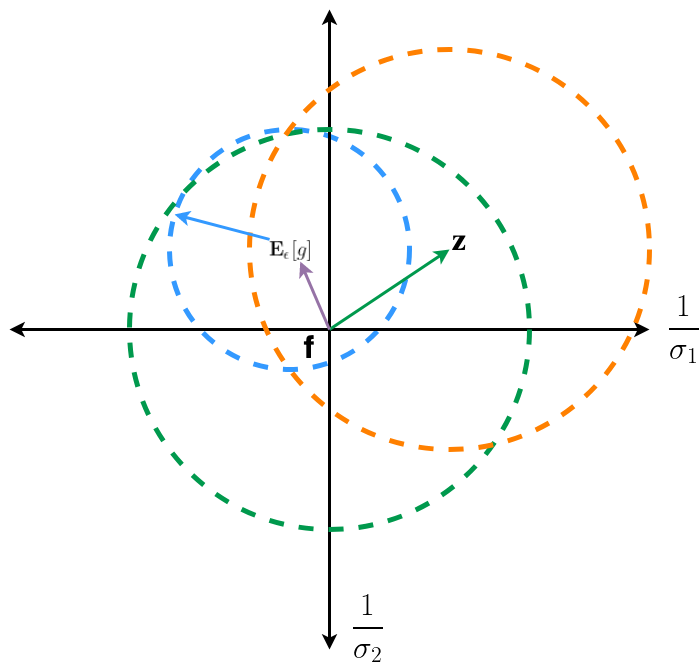
\includegraphics[width=0.75\textwidth]{diagonal_basis_2d_estimators_diagram.png}
  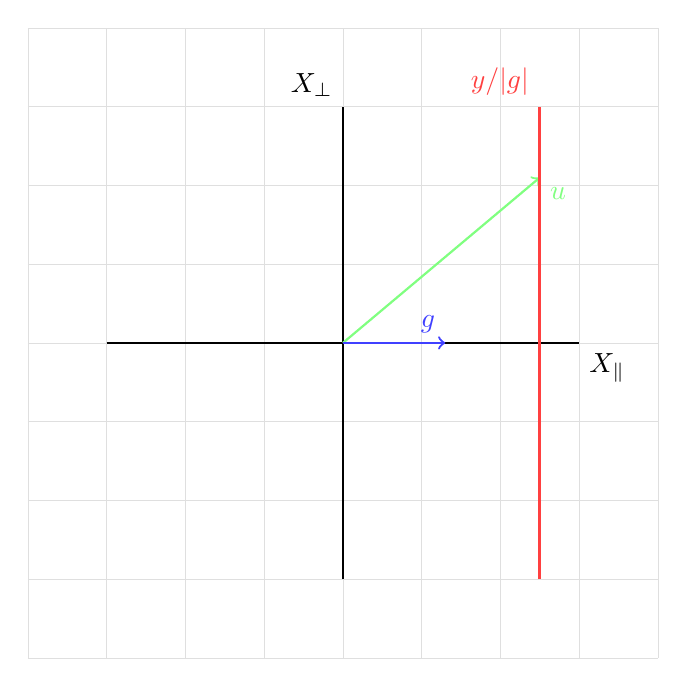
\begin{tikzpicture}
      \draw[step=1cm,gray!25!,very thin] (-4,-4) grid (4,4);
      \draw[thick] (-3,0) -- (3,0) node[anchor=north west] {$X_\parallel$};
      \draw[thick] (0,-3) -- (0,3) node[anchor=south east] {$X_\perp$};
      \draw[green!50,thick,->] (0,0) -- (2.5,2.1) node[anchor=north west] {$u$};
      \draw[blue!75,thick,->] (0,0) -- (1.3, 0) node[anchor=south east] {$g$};
      \draw[red!75,very thick] (2.5,-3) -- (2.5, 3) node[anchor=south east] 
        {$y/|g|$};
  \end{tikzpicture}
  \caption{A linear model in a two-dimensional space is constrained by a single data point $y$. Once the vector $g$ is given, the model is fully specified by the vector $u$, \viz\ $y=g^T u$. All models $u$ along the vertical red line reproduce exactly the data point. In the absence of prior knowledge, every model along that one-dimensional subspace is a legitimate solution of the inverse problem, which is clearly underdetermined.}
  \label{fig:2dexample}
\end{figure}
%
For simplicity we are going to assume that the prior on $\modelvec$ is also a
multi-dimensional Gaussian, centred at $0$ with covariance matrix
$\modelpriorcov$. In this case the posterior distribution can be written as
\begin{equation}
  \label{eq:GaussPostExplicit}
    \pi_{X}^\fwdobsop(\modelvec) 
    \propto \exp \left[
      -\frac{1}{2\gamma^2} \left|\obs - (g^T \modelvec) \right|^2 - \frac12 \left|\modelvec\right|_{\modelpriorcov}^2 
    \right]\, ,
\end{equation}
which is still a Gaussian distribution for $\modelvec$. The mean and covariance
are respectively
\begin{align}
  m &= \frac{(\modelpriorcov g) \obs}{\gamma^2 + (g^T \modelpriorcov g)}\, , \\
  \Sigma &= \modelpriorcov - 
  \frac{(\modelpriorcov g) (\modelpriorcov g)^T}{\gamma^2 + (g^T \modelpriorcov g)}\, .
\end{align}
Because the argument of the exponential is a quadratic form, the mean of the
distribution coincides with the MAP estimator. Hence in this case a fit that
minimises the $\chi^2$ of the data to the theory prediction yields exactly the
mean of the posterior distribution. It is instructive to look at these
quantities in the limit of infinitely precise data, \ie\ in the limit $\gamma\to
0$:
\begin{align}
  m_\star &= 
  \lim_{\gamma\to 0} m
  = \frac{(\modelpriorcov g) \obs}{(g^T \modelpriorcov g)}\, , \\
  \Sigma_\star &= 
  \lim_{\gamma\to 0} \Sigma 
  = \modelpriorcov - 
  \frac{(\modelpriorcov g) (\modelpriorcov g)^T}{(g^T \modelpriorcov g)}\, .
\end{align}
These values satisfy
\begin{align}
  (g^T m_\star) = \obs \, , \\
  (\Sigma_\star g) = 0 \, ,
\end{align}
which shows that the mean of the distribution is such that the data point is
exactly reproduced by the model, and that the uncertainty in the direction
defined by $g$ vanishes. It should be noted that the uncertainty in directions
perpendicular to $g$ does not vanish and is determined by a combination of the
prior and the model, \viz\ $\modelpriorcov$ and $g$ in our example. This is a
particular example of a more general feature: for underdetermined systems the
information from the prior still shapes the probability distribution of the
solution even in the limit of vanishing statistical noise.  

It is interesting to analyse what happens when the prior on the model is
removed. For this purpose we can start from a covariance in model space that is
proportional to the identity matrix, 
\begin{equation}
  \label{eq:DiagCovSigma}
  \modelpriorcov = \sigma \mathbb{1}\, ,
\end{equation}
and take the limit $\sigma \to \infty$. In this limit
\begin{equation}
  \label{eq:LargeSigmaLimit}
  m_\star = y \frac{g}{(g^T g)}\, ,
\end{equation}
while the posterior covariance becomes
\begin{equation}
  \label{eq:ExplcitCov}
  \Sigma_\star= \sigma \left(
    \mathbb{1} - \frac{g g^T}{(g^T g)}
  \right)\, .
\end{equation}
This covariance is the projector on the subspace orthogonal to $g$ multiplied by
$\sigma$. In the simple two-dimensional example depicted in
Fig.~\ref{fig:2dexample}, choosing the direction of $g$ as one of the basis
vector, we obtain
\begin{equation}
  \label{eq:ExplCovTwo}
  \Sigma_\star = 
  \begin{pmatrix}
    0 & \\
    & \sigma
  \end{pmatrix}\, ,
\end{equation}
which shows that the error in the $g$ direction vanishes, while the error in the
orthogonal subspace diverges as we remove the prior. 

\paragraph{Overdetermined system}
We are now going to consider an example of an overdetermined system and discuss
again the case of small observational noise. We consider $\ndata\geq 2$ and
$\nmodel=1$, with a linear forward map such that
\begin{equation}
 \label{eq:OverDetForwMap}
 \obs = g \modelvec  + \obsnoise\, ,
\end{equation} 
where $\obsnoise$ is an $\ndata$-dimensional Gaussian variable with a diagonal
covariance $\gamma^2 \mathbb{1}$, and $\mathbb{1}$ denotes the identity matrix.
For simplicity we are going to assume a Gaussian prior with unit variance for
$\modelvec$, which yields for the posterior distribution:
\begin{equation}
  \label{eq:OverDetPost}
  \pi_{X}^\fwdobsop(\modelvec) 
    \propto 
    \exp\left(
      -\frac{1}{2\gamma^2} \left| \obs - g \modelvec \right|^2
      -\frac12 \modelvec^2
    \right)\, .
\end{equation} 
The posterior is Gaussian and we can easily compute its mean and variance: 
\begin{align}
  m &= \frac{(g^T \obs)}{\gamma^2 + |g|^2} \, , \\
  \sigma^2 &=
    \frac{\gamma^2}{\gamma^2 + |g|^2}\, .
\end{align}
In this case, in the limit of vanishing observational noise, we obtain
\begin{align}
  m_\star &= \frac{(g^T \obs)}{|g|^2} \, ,\\
  \sigma_\star^2 &= 0\, .
\end{align}
The mean is given by the weighted average of the datapoints, which is also the
solution of the $\chi^2$ minimization
\begin{equation}
  m_\star = \arg\min_{\modelvec\in\real} \left|\obs - g \modelvec\right|^2\, .
\end{equation}
Note that in this case the variance $\sigma_\star$ vanishes independently of the
prior. In the limit of small noise, the distribution tends to a Dirac delta
around the value of the MAP estimator.  

\subsection{Linear Problems}
\label{sec:LinProbs}

Linear problems in finite-dimensional spaces are characterized by a simple
forward law, 
\begin{equation}
  \label{eq:MatrixG}
  \obs = \linmap \modelvec\, ,
\end{equation}
where $\linmap$ is a matrix. In this framework one can readily  derive
analytical solutions that are useful to understand the main features of the
Bayesian approach. Assuming that the priors are Gaussian again, the cost
function $S(\modelvec)$ is a quadratic function of $\modelvec$,
\begin{align}
  \label{eq:CostLinGauss}
  S(\modelvec) &= 
  \left(\linmap \modelvec - \obspriorcent \right)^T \obspriorcov^{-1} 
  \left(\linmap \modelvec - \obspriorcent \right) + 
  \left( \modelvec - \modelpriorcent \right)^T \modelpriorcov^{-1} \left(\modelvec - \modelpriorcent \right) \\
  &= 
  \left(\modelvec - \modelpostcent\right) \modelpostcov^{-1}
  \left(\modelvec - \modelpostcent\right) + \mathrm{const}\, ,
\end{align} 
where
\begin{align}
  \label{eq:PostParamsCov}
  \modelpostcov^{-1} &= 
  \left(
    \linmap^T \obspriorcov^{-1} \linmap + \modelpriorcov^{-1}
  \right)\, , \\
  \label{eq:PostParamsMean}
  \modelpostcent &=
  \modelpostcov  \left(
    \linmap^T \obspriorcov^{-1} \obspriorcent + \modelpriorcov^{-1} \modelpriorcent
  \right)\, .
\end{align}
The case where we have no prior information on the model is recovered by taking
the limit $\modelpriorcov^{-1} \to 0$, which yields
\begin{align}
  \label{eq:NoPriorLinModel}
  \modelpostcov^{-1} &= 
  \left(
    \linmap^T \obspriorcov^{-1} \linmap
  \right)\, , \\
  \modelpostcent &=
  \modelpostcov  \left(
    \linmap^T \obspriorcov^{-1} \obspriorcent 
  \right)\, . \label{eq:NoPriorLinModelCov}
\end{align}
The action of $\obspriorcov^{-1}$ on the vector of observed data $\obspriorcent$
is best visualised using a spectral decomposition
\begin{equation}
  \label{eq:CDSpecDec}
  \obspriorcov^{-1} = \sum_n \frac{1}{\sigma_n^2} P_n\, ,
\end{equation}
where $P_n$ denotes the projector on the $n$-th eigenvector of $\obspriorcov$,
and $\sigma_n^2$ is the corresponding eigenvalue. The action of
$\obspriorcov^{-1}$ is to perform a weighted average of the components of
$\obspriorcent$ in the directions of the eigenvectors of $\obspriorcov$.

An explicit expression for the posterior distribution of data can be obtained
from the joint distribution by marginalising over the model input $\modelvec$:
\begin{align}
  \label{eq:PosteriorDataSpace}
  \pi_{Y}&^\fwdobsop(\obs|\obspriorcent,\obspriorcov,\modelpriorcent,\modelpriorcov)
  = \int du\, 
  \pi^\fwdobsop(\obs,\modelvec|\obspriorcent,\obspriorcov,\modelpriorcent,\modelpriorcov) \nonumber\\
  &\propto \exp\left(
    -\frac12 \left(\obs - \obspostcent\right)^T \obspostcov^{-1}
    \left(\obs - \obspostcent\right)
  \right)\, ,
\end{align}
where
\begin{align}
  \label{eq:PosteriorDataParamsMean}
  \obspostcent &= \linmap \modelpostcent\, , \\
  \label{eq:PosteriorDataParamsCov}
  \obspostcov &= \linmap \modelpostcov \linmap^T\, .
\end{align}
Note that this is the naive error propagation from the covariance of the model,
$\modelpostcov$, to the space of data. 

\paragraph{Posterior distribution of unseen data}

In real-life cases we are also interested in the posterior distribution of a set
of data that have not been included in the fit. Because different datasets are
described by the same theory, the knowledge of one dataset will inform our
knowledge of the underlying theory -- \ie\ we will determine a posterior
distribution for the model. That new knowledge about the model will then
propagate to any other -- unseen -- set of data, even if the experiments are
completely unrelated. In the Bayesian framework that we have developed, this
situation can be modeled by having two independent sets of data $y$ and $y'$,
for which we have a prior distribution 
\begin{align}
  \label{eq:JointIndepDataPrior}
  \pi_{Y}^0&\left(y,y'|y_0,C_{Y},y'_0,C'_{Y}\right) 
   = \pi_{Y}^0\left(y'|y'_0,C'_{Y}\right) \pi_{Y}^0\left(y|y_0,C_{Y}\right) \nonumber \\
  & \propto 
  \exp\left[-\frac12 \left(y'-y'_0\right)^T (C'_{Y})^{-1} 
  \left(y'-y'_0\right)\right]\,\times \nonumber\\
  &\quad\exp\left[-\frac12 \left(y-y_0\right)^T (C_{Y})^{-1} 
  \left(y-y_0\right)\right]\, .
\end{align}
Note that the prior distribution is factorised as the product of individual
distributions for $y$ and $y'$ since the datasets are assumed to be independent.
Following the derivation above, we can write the joint distribution for the data
and the model 
\begin{align}
  \label{eq:JointModelData}
  \pi&^\fwdobsop(y,y',u) 
  \propto \nonumber \\
  &\pi_{Y}^0(y,y'|y_0,C_{Y},y'_0,C'_{Y}) 
  \pi_{X}^0(u) 
  \delta\left(y - \mathcal{G}u\right)
  \delta\left(y'- \mathcal{G}'u\right)\, .
\end{align}
Because both sets of data are derived from the same model $u$, the joint
distribution above introduces a correlation between the data sets. The same
model $u$ appears in both delta functions in the equation above. We can now
marginalise with respect to the dataset $y$, 
\begin{equation}
  \label{eq:MarginaliseDatasetY}
  \begin{split}
    \pi&(y',u) 
    \propto 
    \exp\left[-\frac12 \left(y'-y'_0\right)^T (C'_{Y})^{-1} 
    \left(y'-y'_0\right)\right]\, \nonumber \\
    &\times \exp\left[-\frac12 \left(u-\tilde{u}\right)^T (\tilde{C}_{X})^{-1} 
    \left(u-\tilde{u}\right)\right] 
     \delta\left(y'- \mathcal{G}'u\right)\, .
  \end{split}
\end{equation}
where $\tilde{C}_{X}$ and $\tilde{u}$ are given respectively in
Eqs.~\ref{eq:PostParamsCov} and \ref{eq:PostParamsMean}. By marginalising again,
this time with respect to the model, we derive the posterior distribution of the
unseen data,
\begin{equation}
  \label{eq:MarginaliseModelU}
  \pi^y_{Y}(y') \propto 
  \exp \left[ 
   \frac12 \left(y' - \tilde{y}'\right)^T
   (\tilde{C}'_{Y})^{-1} 
   \left(y' - \tilde{y}'\right)
   \right]\, ,
\end{equation}
where
\begin{align}
  \label{eq:lineone}
  \tilde{C}'_{Y} 
  &= \mathcal{G}' \tilde{C}'_{X} \mathcal{G}'^{T} \\
  \label{eq:linetwo}
  \tilde{y}'
  &= \mathcal{G}' \tilde{u}'\, ,
\end{align}
and we have introduced the variables $\tilde{u}'$ and $\tilde{C}'_{X}$,  
\begin{align}
  \label{eq:ModelPostSequential}
  \tilde{C}_{X}'^{-1} 
  &= \mathcal{G}'^T C_{Y}'^{-1} \mathcal{G}' + \tilde{C}_{X}^{-1} \\
  \label{eq:ModelPostSequentialTwo}
  \tilde{u}' 
  &= \tilde{C}'_{X} \left(
    \mathcal{G}'^T C_{Y}'^{-1} y_0' + \tilde{C}_{X}^{-1} \tilde{u} 
    \right) \, .
\end{align}
The variables $\tilde{C}_{X}$ and $\tilde{u}$ have been defined above. We repeat
their definition here in order to have all the necessary equations collected
together: 
\begin{align}
  \label{eq:linethree}
  \tilde{C}_{X}^{-1}
  &= \mathcal{G}^T C_{Y}^{-1} \mathcal{G} + C_{X}^{-1} \\
  \label{eq:linefour}
  \tilde{u}
  &= \tilde{C}_{X} \left(
    \mathcal{G}^T C_{Y}^{-1} y_0 + C_{X}^{-1} u_0
  \right)\, .
\end{align}
Eqs.~\ref{eq:lineone}, \ref{eq:linetwo}, \ref{eq:ModelPostSequential},
\ref{eq:ModelPostSequentialTwo}, \ref{eq:linethree} and \ref{eq:linefour} yield
the central value and the variance of the posterior distribution of unseen data
as a function of $y_0$, $y_0'$, $C_Y$, $C_Y'$, $u_0$ and $C_X$. 

\paragraph{A comment on non-linear models}

The linear models that we have discussed so far may look over-simplified at
first sight. In practice, it turns out that non-linear models can often be
linearised around the central value of the prior distribution, 
\begin{equation}
  \label{eq:LinU0}
  \fwdobsop(\modelvec) = \fwdobsop(\modelpriorcent) + G \left(\modelvec - \modelpriorcent\right) + \ldots\, ,
\end{equation}
where 
\begin{equation}
  \label{eq:FirstDerU0}
  G^i_\alpha = \left. \frac{\partial \fwdobsop^i}{\partial u_\alpha} \right|_{\modelpriorcent}\, ,
\end{equation}
and we have neglected higher-order terms in the expansion of
$\fwdobsop(\modelvec)$.

If these terms are not negligible, another option is to find the MAP estimator,
and then expand the the forward map around it, which yields equations very
similar to the previous ones, with $\modelpriorcent$ replaced by $u_*$. If the
posterior distribution of $u$ is sufficiently peaked around the
MAP estimator, then the linear approximation can be sufficiently accurate. 


\subsection{The infinite-dimensional case}
\label{sec:infin-dimens-case}

In the finite-dimensional case, where the probability measures are specified by
their densities with respect to the Lebesgue measure,
Eq.~(\ref{eq:BayesThmInversePosterior}) can be rephrased by saying  that $\rho$
is the Radon-Nikodym derivative of the probability measure $\mu^\fwdobsop$ with
respect to $\mu_0$, \viz
\begin{align}
  \label{eq:RadonNikodym}
  \frac{d\mu^\fwdobsop}{d\mu^0} (\modelvec) \propto \rho(\obs-\fwdobsop(\modelvec))\, .
\end{align}
Using the fact that the density $\rho$ is a positive function, we can rewrite 
\begin{align}
  \label{eq:PotentialDef}
  \rho(\obs-\fwdobsop(\modelvec)) = \exp\left(-\Phi(\modelvec;\obs)\right)\, ,
\end{align}
and therefore
\begin{align}
  \label{eq:RadonNikodymTwo}
  \frac{d\mu^\fwdobsop}{d\mu^0} (\modelvec) \propto \exp\left(-\Phi(\modelvec;\obs)\right)\, .
\end{align}
In finite-dimensional spaces, the three equations above are just definitions
that do not add anything to the above discussion in terms of probability
densities. Their interest resides in the fact that the last expression,
Eq.~(\ref{eq:RadonNikodymTwo}), can be properly defined when $\modelspace$ is
infinite-dimensional, allowing a rigorous extension of the Bayesian formulation
of inverse problems to the case of infinite-dimensional spaces. 

Summarising the details of probability measure in infinite-dimensional spaces,
is beyond the scope of this work. Adopting instead a heuristic approach, we can
say that a function $f$ is a random function if $f(x)$ is a random variable for
all values of $x$. Since the values of the function at different values of $x$
can be correlated, a random function is fully characterised by specifying the
joint probability densities
\begin{equation}
  \label{eq:RandomFuncJointProb}
  \pi\left(
    f_1, \ldots, f_n; x_1, \ldots x_n
  \right)\, ,
\end{equation}
where $f_i=f(x_i)$, for all values of $n$, and all values of $x_1, \ldots, x_n$.
This infinite set of finite-dimensional densities allows the definition of a
probability measure. 

For a Gaussian random function, these densities only depend on a mean value
function $m(x)$ and a covariance $C(x,x')$. The probability densities for the
variables $f_i$, for any value of $n$ is 
\begin{align}
  \label{eq:GaussianFunctC}
  \pi&\left(f_1, \ldots, f_n; x_1, \ldots, x_n\right) 
  \propto \nonumber \\ 
  &\exp \left[ 
      -\frac12 \sum_{ij} \left(f_i - m_i\right) C^{-1}(x_i,x_j) \left(f_j - m_j\right)
    \right]\, .
\end{align} 
The covariance $C$ is such that
\begin{equation}
  \label{eq:CovFunctInt}
  C(x,x') = \int df\, df'\, \left(f - m(x)\right) \left(f'-m(x')\right)
    \pi\left(f,f';x,x'\right)\,,
\end{equation}
which shows that the two-point probability density determines all the other
distributions. 

\paragraph{Functional linear problems} This formalism allows us to formulate a
Bayesian solution of the inverse problem 
\begin{equation}
  \label{eq:BayesLinearInverse}
  y^i = \int dx\, G^i(x) u(x)\, ,
\end{equation}
where $y^i$ is a discrete set of observables and $u(x)$ is a random function,
with a Gaussian prior with mean $u_0(x)$ and covariance $C_{X}(x,x')$. The
vector of observed values is denoted $y_0$, and we assume that the prior
distribution of $y$ is a Gaussian centred at $y_0$ with covariance $C_{Y}$.

Similarly to the finite-dimensional case, the Bayesian solution yields a
Gaussian random function for the posterior distribution of the solution $u(x)$.
In order to characterise the posterior Gaussian distribution we need explicit
expressions for its mean and its covariance. Introducing the matrix
\begin{equation}
  \label{eq:Smatrix}
  S^{ij} =
  \int dx dx'\, G^i(x) C_{X}(x,x') G^j(x') + C_{Y}^{ij}\, ,
\end{equation}
and its inverse $T^{ij}=\left(S^{-1}\right)^{ij}$, the posterior Gaussian field
is centred at
\begin{align}
  \label{eq:PostMeanFunc}
  \tilde{u}&(x) = u_0(x) + \int dx'\, C_{X}(x,x') \nonumber \\ 
  &\times G^i(x') T^{ij} \left(
    y_0^j - \int dx''\, G^j(x'') u_0(x'') 
  \right)\, ,
\end{align}
which is the expected generalization of the finite-dimensional example discussed
above. Interestingly, this can be rewritten as
\begin{equation}
  \label{eq:TowardsBackus}
  \tilde{u}(x) = u_0(x) + 
  \int dx'\, C_{X}(x,x') \psi(x')\, ,
\end{equation}
where 
\begin{eqnarray}
  \label{eq:PsiDef}
  \psi(x) = G^i(x) \delta y^i\, ,
\end{eqnarray}
and the weighted residuals are given by
\begin{equation}
  \label{eq:DeltaYDef}
  \delta y^i = T^{ij} \left(
  y_0^j - \int dx'\, G^j(x') u_0(x')
  \right)\, .
\end{equation}
Defining 
\begin{equation}
  \label{eq:CapitalPsi}
  \Psi^i(x) = \int dx'\, C_{X}(x,x') G^i(x')\, ,
\end{equation}
the posterior covariance can be written as
\begin{equation}
  \label{eq:PostCovFunc}
  \tilde{C}_{X}(x,x') = 
  C_{X}(x,x') - \Psi^i(x) T^{ij} \Psi^j(x')\, .
\end{equation}

It is instructive to compare the Bayesian result summarised above with the
method proposed by Backus and Gilbert~\cite{BackusGilbert1968} to solve the same
inverse problem. Assuming that there exists an unknown 'true' model $\utrue$,
such that the observed data are
\begin{equation}
  \label{eq:BackStart}
  y_0^i = \int dx\, G^i(x) \utrue(x)\, ,
\end{equation}
we look for an estimate $\uest$ of the true solution in the form
\begin{equation}
  \label{eq:BackAnsatz}
  \uest(x) = Q^i(x) y^i_0\, ,
\end{equation}
so that the problem is now recast as finding the functions $Q^i(x)$.
Using Eq.~\ref{eq:BackStart} we obtain
\begin{equation}
  \label{eq:BackFilter}
  \uest(x) = \int dx' R(x,x') \utrue(x')\, , 
\end{equation}
which states that with a finite amount of data we can only resolve a filtered
version of the true solution. The kernel $R$ is given by
\begin{equation}
  \label{eq:BackKernel}
  R(x,x') = Q^i(x) G^i(x')\, .
\end{equation}
The coefficient functions $Q^i(x)$ can be chosen so that the kernel is as close as possible
to a delta function,
\begin{equation}
  \label{eq:BackDelta}
  R(x,x') \simeq \delta(x,x') ~~ \Longrightarrow ~~
  \uest \simeq \utrue\, .
\end{equation}
Approximating the delta function can be achieved by minimising 
\begin{equation}
  \label{eq:BackDeltaness}
  \int dx'\, \left(
    R(x,x') - \delta(x-x')
  \right)^2\, ,
\end{equation}
which yields
\begin{equation}
  \label{eq:BackSolution}
  Q^i(x) = \left(S^{-1}\right)^{ij} G^j(x)\, ,
\end{equation}
where 
\begin{equation}
  \label{eq:BackSMatrix}
  S^{ij} = \int dx\, G^i(x) G^j(x)\, .
\end{equation}
The interesting observation is that the central value of the Bayesian solution
presented above reduces to the Backus-Gilbert $\uest$ in the case where $u_0$ 
is just white noise and therefore
\begin{equation}
  \label{eq:BackComparison}
  C_{X}(x,x') = \delta(x-x')\, .
\end{equation}
The connections between the Bayesian treatment and the Backus-Gilbert solution
and its regulated variations, deserves further investigations, which we defer to
future studies. Note that the Bayesian solution allows a variety of priors to be
explicitly declared and compared to the Backus-Gilbert solution. 
\section{Data and Fitting}

When fitting experimental data we vary the parameters of a set of PDF replicas
at the initial scale such that the $\chi^2$ is minimised between the
corresponding theory predictions and a generated pseudodata replica. A set of
PDFs usually refers to a set of seperate continuous functions, one for each
flavour of PDF in a particular basis. In this specific study, fits performed
with \nfit\ parameterise the set of PDFs as a single neural network which takes
as input $x$ and $\ln x$ and returns 8 outputs, one for each flavour in the
fitting basis, multiplied by some preproccessing exponents. The output for a
single flavour $j$ is
\begin{equation}
    NN(x, \ln x)_j * x^{1-\alpha_j} * (1-x)^{\beta_j},
\end{equation}
where each flavour has it's own preproccessing exponents $\alpha$ and $\beta$,
parameters that are varied in these fits, and $NN(x, \ln x)_j$ is the
$j^{\rm th}$ output from the neural network. The pseudodata replica is generated
through Monte Carlo sampling according to the experimental uncertainty, by
applying noise to the experimental
central values. After fitting many sets of PDF replicas (usually of order 100 sets),
each set to an independently generated pseudodata replica, we have an ensemble of
PDF replicas which is a sample of the probability distribution of the PDF given
the data. The aim of this methodology, is to propagate the various sources of
uncertainty involved with fitting PDFs into the functional PDF space.

If we consider experimental data which we assume
to be multigaussian then the experimental central values, $\levone$, are given by
\begin{equation}
    \levone_{i} = \law_i + \shift_i,
\end{equation}
where $i$ is the index of the data point.
In other words, the experimental values have been shifted away from the true
values given by nature, $\law$, by some shift, $\shift$. The vector of shifts
is drawn from
the multigaussian $\mathcal{N}(0, \cov)$ where $\cov$ is the experimental
covariance matrix. The fitted pseudodata is obtained by adding Monte Carlo
noise, $\noise^{\repind}$, on top of the experimental central values
\begin{equation}
    \levtwo^{\repind}_{i} = \law_i + \shift_i + \noise^{\repind}_{i},
\end{equation}
where the replica index $k$ refers to each replica having a noise vector drawn
independently from $\mathcal{N}(0, \cov)$. The sampling of pseudodata permits
correlations between individual data points through the covariance matrix,
but not between different replicas or fits.

The $\chi^2$ which is minimised for replica $k$ is then given by
\begin{equation}
    \repchis = \frac{1}{\ndata} \sum_{ij} \diffreptwo_i \invcov{ij} \diffreptwo_j,
\end{equation}
where $\model^{\repind}_i$ is the prediction for $i^{\rm th}$ datapoint, from
the $k^{\rm th}$ set of PDFs. After fitting many replicas, the quality of a fit
is often determined by considering the $\chi^2$ between the experimental central
values and the expectation value of the theory predictions
\begin{equation}\label{eq:centralchi2}
    \chi^2 = \frac{1}{\ndata} \sum_{ij} \diffcentone_i \invcov{ij} \diffcentone_j,
\end{equation}
where $\erep{\cdot}$ denotes the mean value across replicas, so $\erep{g}$ is
the mean of the theory predictions across replicas. This $\chi^2$ is a measure
of the difference between the expectation value of the prediction and the
experimental central values in units of the covariance.

In a fit to experimental data we are limited to this quantity because we don't
have knowledge of the underlying theory predictions of nature $\law$. In a
closure test we use a pre-existing PDF as proxy for $\law$ and then
generate both $\shift$ and $\noise$ from $\mathcal{N}(0, \cov)$, emulating the
different levels of data. The underlying theory predictions are referred to as
level zero data. We refer to the shifted central values as level one data, the
underlying law plus a level one shift. The pseudodata which a given replica fits
is then referred to as level two data.

\section{Data space estimators} 
\label{sec:ClosureEstimators}

In order to perform a quantitative analysis of the results obtained in the
closure tests, we discuss several estimators, which are computed from the
outcome of the closure test fits. These results depend on the pseudo-data that
have been generated and therefore are stochastic variables which can fluctuate.
The values of the estimators on a single replica will not tell anything about
the quality of our fits: we need to understand their probability distributions
in order to validate our fitting procedure. We begin this section by defining
estimators in data space, \ie\ estimators that are computed from the model
predictions for a set of experimental data points. Having defined the
estimators, we define criteria to characterise faithful uncertainties. We
conclude this section with a discussion of the predictions that can be obtained
for these estimators in the case of a linear model, where analytical
calculations can be performed. As we already saw in the previoius Section, the
analytical results cannot be applied directly to the NNPDF fits, but they are
useful examples that illustrate the expected behaviour of these quantities.

\subsection{Deriving the data space estimators}
\label{sec:ClosureEstimatorsDerivation}

For a given model $\modelvecrep$, obtained from fitting the $k$-th replica, we
start by defining the model error as the $\chi^2$ between the model predictions
and some data central values $\testset{\obspriorcent}$, normalised by the number
of data points
\begin{equation}
    \label{eq:chi2kereponerep}
    \frac{1}{\ndata} 
        \left( \testset{\fwdobsop}\left(\modelvecrep\right) - \testset{\obspriorcent} \right)^T
        \testset{\obspriorcov}^{-1}
        \left( \testset{\fwdobsop}\left(\modelvecrep\right) - \testset{\obspriorcent} \right)\, ,
\end{equation}
and we purposely denoted the data which the model error is evaluated on as
$\testset{\obspriorcent}$, as opposed to the training data $\obspriorcent$,
which is used to determine the model parameters. The corresponding covariance is
denoted $\testset{\obspriorcov}$. Note that in Eq.~\ref{eq:chi2kereponerep},
$\testset{\obspriorcent}$ is a stochastic variable, but also $\modelvecrep$ is a
stochastic variable, with its pattern of fluctuations, since the fitted model
depends on the data $\pseudodat^{\repind}$ that enter the fit. We define the
model error $\eout$ on the set of data $\testset{\obspriorcent}$ by taking the
average over the models,
\begin{equation}
    \label{eq:chi2kerep}
    \eout = \frac{1}{\ndata} \emodel{
        \left( \testset{\fwdobsop}\left(\modelvecrep\right) - \testset{\obspriorcent} \right)^T
        \testset{\obspriorcov}^{-1}
        \left( \testset{\fwdobsop}\left(\modelvecrep\right) - \testset{\obspriorcent} \right)
    }\, ,
\end{equation}
where we defined the expectation value over the ensemble of model replicas as
\begin{equation}
    \emodel{x} \equiv \frac{1}{\nreps} \sum_{k=1}^{\nreps} x^{(k)} \, .
\end{equation}
We could of course set $\testset{\obspriorcent} = \obspriorcent$ and evaluate
the model performance on the fitted data however, as is common in machine
learning literature, we intend to use a separate set of test data. Ideally we
would choose $\testset{\obspriorcent}$ such that $\testset{\obspriorcent}$ and
$\obspriorcent$ are statistically independent, as in
Eq.~\ref{eq:JointIndepDataPrior}. This is achieved by choosing the split such
that the experimental covariance matrix is block diagonal:
\begin{equation}
    \modelpriorcov^{\rm total} =
    \begin{bmatrix}
        \modelpriorcov  & 0  \\ 
        0  & \testset{\modelpriorcov}  \\ 
    \end{bmatrix}\, .
\end{equation}
% In the context of a closure test, $\eout$ is a stochastic quantity which
% depends both on the training data, through the ensemble of MAP estimators, and
% the test data.

It is useful to perform a decomposition of Eq.~\ref{eq:chi2kerep}, following
usual manipulations of the likelihood function associated with least-squares
regression in~\cite{mlforphysics}. Least-squares regression is a special case of
minimum likelihood estimation, where the uncertainty on each data point is equal
in magnitude and uncorrelated. Here we review the decomposition in the more
general framework of data whose uncertainty is multigaussian. Starting with
Eq.~\ref{eq:chi2kerep} (evaluated on the ideal test data), we can complete the
square
\begin{equation}
    \begin{split}
    \label{eq:EoutDecomposition}
        &\eout = \frac{1}{\ndata} \emodel{
            \left( \testset{\fwdobsop}\left(\modelvecrep\right) - \testset{\law} \right)^T
            \testset{\obspriorcov}^{-1}
            \left( \testset{\fwdobsop}\left(\modelvecrep\right) - \testset{\law} \right)
        } + \\
        &+ \emodel{
            \left( \testset{\law} - \testset{\obspriorcent} \right)^T
            \testset{\obspriorcov}^{-1}
            \left( \testset{\law} - \testset{\obspriorcent} \right)
        }+ \\
        &+ 2 \emodel{
            \left( \testset{\fwdobsop}\left(\modelvecrep\right) - \testset{\law} \right)^T
            \testset{\obspriorcov}^{-1}
            \left(\testset{\law} - \testset{\obspriorcent} \right)
        }\, .
    \end{split}
\end{equation}
Let us now discuss these terms one by one, starting from the last two. The
second term is the shift associated with evaluating the model error on noisey
test data and the final term is a cross term which we will deal with later. We
therefore focus next on further decomposing the first term,
\begin{equation}
    \begin{split}
        &\emodel{
            \left( \testset{\fwdobsop}\left(\modelvecrep\right) - \testset{\law} \right)^T
            \testset{\obspriorcov}^{-1}
            \left( \testset{\fwdobsop}\left(\modelvecrep\right) - \testset{\law} \right)
        } = \\
        &= \emodel{
            \left( \testset{\fwdobsop}\left(\modelvecrep\right) - 
            \emodel{\testset{\fwdobsop}\left(\modelvecrep\right)} \right)^T
            \testset{\obspriorcov}^{-1}
            \left( \testset{\fwdobsop}\left(\modelvecrep\right) - 
            \emodel{\testset{\fwdobsop}\left(\modelvecrep\right)} \right)
        } + \\
        &+ \left( \emodel{\testset{\fwdobsop}\left(\modelvecrep\right)} - \testset{\law} \right)^T
        \testset{\obspriorcov}^{-1}
        \left( \emodel{\testset{\fwdobsop}\left(\modelvecrep\right)} - \testset{\law} \right)\, ,
    \end{split}
\end{equation}
where we have used the fact that the second term is constant across replicas and
the cross term that arises in this decomposition is zero when the expectation
value across replicas is taken. The first term in this expression we call the
{\em variance} and the second term is the {\em bias}.

As previously mentioned $\eout$ should be considered a stochastic estimator, in
theory we could take the expectation value across training data $\obspriorcent$ and
test data $\testset{\obspriorcent}$, the latter of which cancels the cross term in
Eq.~\ref{eq:EoutDecomposition}. The final result of that would be
\begin{equation}\label{eq:ExpectedBiasVariance}
    \mathbf{E}_{\obspriorcent, \testset{\obspriorcent}}[\eout] =
    \mathbf{E}_{\obspriorcent}[{\rm bias}] + 
    \mathbf{E}_{\obspriorcent}[{\rm variance}] +
    \mathbf{E}_{\testset{\obspriorcent}}[{\rm noise}]\, .
\end{equation}
We are not interested in the observational noise term, since it is
independent of the model and in the limit of infinite test data
$\mathbf{E}_{\testset{\obspriorcent}}[{\rm noise}] \to 1$.
The two estimators of interest are independent of
the test data, and therefore we only need to take the expectation value over
the training data.

\paragraph{Multiple closure fits}
In practical terms, taking the expectation value across the training data can
be achieved by running multiple closure fits, each with a different
observational noise vector $\obsnoise$, and taking the average i.e.
\begin{equation}
    \mathbf{E}_{\obspriorcent}[ x ] = \frac{1}{\nfits} \sum_{j=1}^{\nfits} x.
\end{equation}
Clearly this is resource intensive, and requires us to perform many fits. In
NNPDF3.0 \cite{nnpdf30}, single replica proxy fits were used to perform a study
of the uncertainties. Here we have expanded the data-space estimators used in
the closure fits and also will be using multiple full replica fits to
calculate various expectation values - made possible by our next generation
fitting code.

\subsection{Geometric Interpretation}

It is possible to interpret the relevant data space estimators geometrically, by
considering a coordinate system where each basis vector corresponds to an
eigenvector of the experimental covariance matrix normalised by the square root
of the corresponding eigenvalue. An example of this is given in
Fig.~\ref{fig:diagram2destimators}, where for simplicity we have considered a
system with just two data points, \ie\ a two-dimensional data space, with a
diagonal covariance. The origin of the coordinate system is the true value of
the observable. The observational noise in these coordinates corresponds to a
unit circle centred in the origin as shown in
Fig.~\ref{fig:diagram2destimators}. If the experimental covariance is faithful,
there is a 68\%  probability that the experimental value $y_0$ is within this
unit circle. Fig.~\ref{fig:diagram2destimators} shows one possible instance of
$y_0$. Repeating the entire fit procedure multiple times requires generating new
sets of experimental data $y_0$. The average over $y_0$ mentioned above, is
precisely the average over multiple fits, restarting the procedure each time
from a new instance of $y_0$.

For a given $y_0$ the replicas are generated as a set of points Gaussianly
distributed around it and therefore, in the limit of a large number of replicas,
68\% of them will fall within a unit circle centred in $y_0$. This is the dashed
circe in the figure. Clearly there is also a 68\% probability that the true
value (\ie\ the origin in our plot) is inside this second circle. The model
predictions, one for each replica, are then a set of points, whose mean is
$E_\epsilon[g]$. The mean squared radius of those points is what we call the
variance. The bias is the l2-norm of the vector between the origin and the mean
of the model predictions. 

A faithful representation of the errors requires that the true value, \ie\ the
origin of the coordinate system in our figure, has 68\% probability of being
within 1$\sigma$ from the central value of the fit, which is given by
$E_\epsilon[g]$. Looking at the figure again, the probability for the origin to
be inside the shaded circle must be 68\%. We will discuss faithful errors in
more detail in the next subsection.
%
\begin{figure}[h!]
    \centering
    %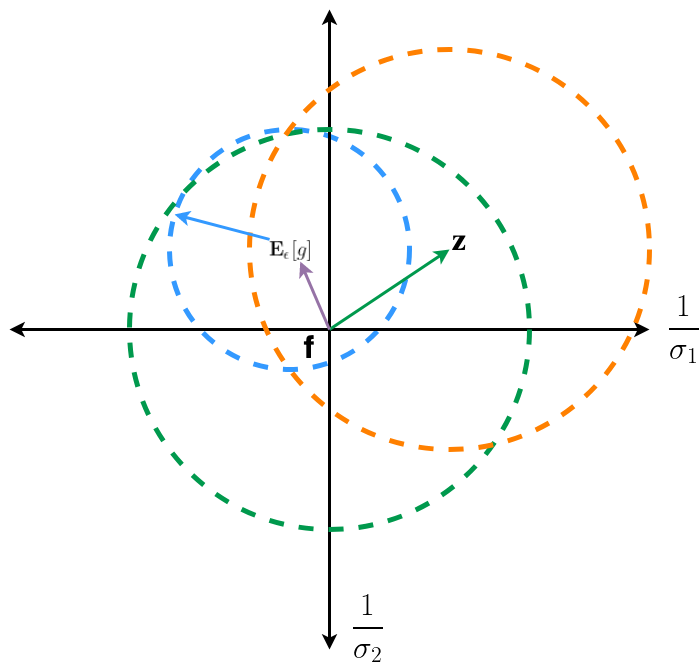
\includegraphics[width=0.75\textwidth]{diagonal_basis_2d_estimators_diagram.png}
    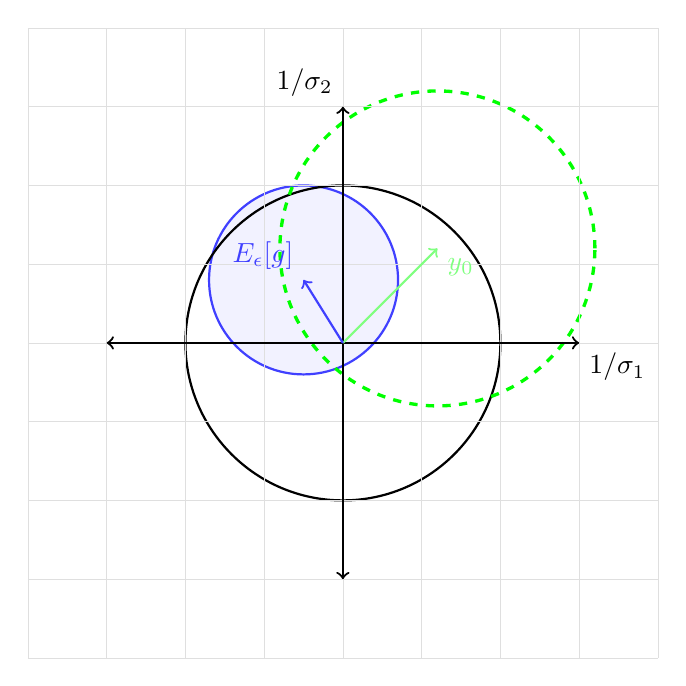
\begin{tikzpicture}
        \draw[blue!75, fill=blue!5, thick] (-0.5, 0.8) circle (1.2 cm);
        \draw[thick] (0,0) circle (2 cm);
        \draw[green, very thick, dashed] (1.2,1.2) circle (2 cm);
        \draw[step=1cm,gray!25!,very thin] (-4,-4) grid (4,4);
        \draw[thick,<->] (-3,0) -- (3,0) node[anchor=north west] {$1/\sigma_1$};
        \draw[thick,<->] (0,-3) -- (0,3) node[anchor=south east] {$1/\sigma_2$};
        \draw[green!50,thick,->] (0,0) -- (1.2,1.2) node[anchor=north west] {$\obspriorcent$};
        \draw[blue!75,thick,->] (0,0) -- (-0.5, 0.8) node[anchor=south east] {$E_\epsilon[g]$};
        \end{tikzpicture}
    \caption{Example of geometric interpretation of closure test estimators.
    The origin
    is the true observable values for each data point. The level one data (or
    experimental central values) are
    shifted away from this by $\obsnoise$. In this example the covariance matrix
    is diagonal, so the eigenvectors correspond to the two data points, the
    square root of the eigenvalues are simply the standard deviation of those
    points. This is without loss of generality because any multivariate distribution
    can be rotated into a basis which diagonalises the covariance matrix.
    The 1-sigma observational noise confidence interval
    is a unit circle centered on the origin. Some closure
    estimators can be understood as l2-norms of the vectors connecting points,
    i.e the bias is the l2-norm of the vector from the origin to the central
    value of the predictions.}
    \label{fig:diagram2destimators}
\end{figure}
%

\subsection{Faithful uncertainties in data space}

The two closure estimators of interest, bias and variance, can be used to
understand faithful uncertainties in a practical sense. If we return to
Eq.~\ref{eq:ExpectedBiasVariance} we can examine both estimators in a more
detail.

\paragraph{Variance}

The {\em variance} in the above decomposition refers to the variance of the
model predictions in units of the covariance
\begin{equation}
    \label{eq:VarDef}
    \begin{split}
        % NOTE: not using \emodel here in order to split line.
        \var &= \frac{1}{\ndata}\mathbf{E}_{\{ \modelvec_* \}} \Big[ \\
            &\left( \testset{\fwdobsop}\left(\modelvecrep\right) - 
            \emodel{\testset{\fwdobsop}\left(\modelvecrep\right)} \right)^T
            \testset{\obspriorcov}^{-1}
            \left( \testset{\fwdobsop}\left(\modelvecrep\right) - 
            \emodel{\testset{\fwdobsop}\left(\modelvecrep\right)} \right)
        \Big] \, ,
    \end{split}
\end{equation}
which can be interpreted as the model uncertainty in the space of the test data.
It is instructive to rephrase Eq.~\ref{eq:VarDef} as
\begin{equation}
    \label{eq:VarDefalternative}
    \var = \frac{1}{\ndata} {\rm Tr} \left[ \covrep \testset{\obspriorcov}^{-1} \right],
\end{equation}
where 
\begin{equation}
    \label{eq:CovRep}
    \covrep = 
    \emodel{
            \left( \testset{\fwdobsop}\left(\modelvecrep\right) - 
            \emodel{\testset{\fwdobsop}\left(\modelvecrep\right)} \right)
            \left( \testset{\fwdobsop}\left(\modelvecrep\right) - 
            \emodel{\testset{\fwdobsop}\left(\modelvecrep\right)} \right)^T
        }
\end{equation}
is the covariance matrix of the predictions from the model replicas. Note that
we can rotate to a basis where $\testset{\obspriorcov}$ is diagonal,
\begin{equation}
    \label{eq:InvCovPrimeDiag}
    \left(\testset{\obspriorcov}^{-1} \right)_{ij} = \frac{1}{\left(\testset{\sigma}_i\right)^2} 
    \delta_{ij}\, ,
\end{equation}
then we can rewrite Eq.~\ref{eq:VarDefalternative} as 
\begin{equation}
    \label{eq:VarianceInterpretation}
    \var = \frac{1}{\ndata}\, \sum_i \frac{\covrep_{ii}}{\left(\testset{\sigma}_i\right)^2}\, .
\end{equation}
The numerator in the right-hand side of the equation above is the variance of
the theoretical prediction obtained from the fitted replicas, while the
denominator is the experimental variance, the average is now taken over
eigenvectors of the experimental covariance matrix. Note that this ratio does
not need to be equal to one, the model error on a given point can be smaller
than the experimental one, since all theoretical estimates are correlated by the
underlying theoretical law. 

% The following needs to be reworded or removed, the use of prior and posterior
% here is confusing because the prior here is nothing to do with the prior
% of the training data but the posterior is only the posterior of the training
% data and instead is the prior of the model when considering the test data..

% If the replicas are sampled from the
% posterior distribution of model, the right-hand side of the
% equation is the average reduction in the variance of the observables between the
% prior distribution, dictated by the experimental covariance, and the posterior
% distribution. The average is computed over the space of test data, \ie\ data
% points that are not seen by the fit. 

\paragraph{Bias}

Similarly, the {\em bias}\ is defined as the difference between the expectation
value of the model predictions and the true observable values in units of the
covariance, \ie 
\begin{equation}
    \label{eq:BiasDef}
    \bias = \frac{1}{\ndata}
    \left( \emodel{\testset{\fwdobsop}\left(\modelvecrep\right)} - \testset{\law} \right)^T
    \testset{\obspriorcov}^{-1}
    \left( \emodel{\testset{\fwdobsop}\left(\modelvecrep\right)} - \testset{\law} \right)\, .
\end{equation}
The smaller the bias, the closer the central value of the predictions is to the
underlying law. In Eq.~\ref{eq:ExpectedBiasVariance}, the expectation value is
taken across the prior distribution of the training data, which yields
\begin{equation}
    \mathbf{E}_{\obspriorcent}[{\rm bias}] = \frac{1}{\ndata}
    {\rm Tr} \left[ \covcent \testset{\obspriorcov}^{-1} \right]\, ,
\end{equation}
where we have introduced $\covcent$ as the covariance of the expectation value
of the model predictions,
\begin{equation}
    \label{eq:CovCentDef}
    \covcent = 
    \mathbf{E}_{\obspriorcent}\left[
        \left( \emodel{\testset{\fwdobsop}\left(\modelvecrep\right)} - \testset{\law} \right)
        \left( \emodel{\testset{\fwdobsop}\left(\modelvecrep\right)} - \testset{\law} \right)^T   
    \right]\, .
\end{equation}
The point is that the bias on the test data is a stochastic variable which
depends on the central value of the training data through $\modelvecrep$. The
matrix $\covcent$ describes the fluctuations of the central value of the model
prediction around the true observable values as we scan different realisations
of the training data. 

It is important to stress the difference between variance and bias. In the case
of the variance, we are looking at the fluctuations of the replicas around their
central value for fixed $\obspriorcent$. This is related to the ensemble of
model replicas we provide as the end product of a fit and can be calculated when
we have one instance of $\obspriorcent$, provided by the experiments. In the
case of the bias we consider the fluctuations of the central value over replicas
around the true theoretical prediction as the values of $\obspriorcent$
fluctuate around $\law$. This latter procedure is only possible in a closure
test, where the underlying true observable is known. The bias as defined here
yields an estimate of the fluctuations of the MAP estimator if we could do
multiple independent instances of their measurements from each experiment.

\paragraph{Bias-variance ratio}

Finally, the {\em bias-variance ratio} is defined as
\begin{equation}
    \label{eq:RatioDef}
    \biasvarratio \equiv \sqrt{\frac{
        \mathbf{E}_{\obspriorcent}[ \bias ]}{
            \mathbf{E}_{\obspriorcent}[ \var ]}}\, ,
\end{equation}
where we have taken the square root, since bias and variance are both mean
squared quantities. The value of $\biasvarratio$ yields a measurement of how
much uncertainties are over or under estimated. If the uncertainties are
completely faithful, then $\biasvarratio = 1$. 
% We note that the relationship
% does not work both ways and $\biasvarratio = 1$ does not necessarily guarantee
% that the uncertainty is faithful. 
%
We note that $\biasvarratio$ is not completely general: it is not a measure
defined in model space and depends on the choice of test data. Therefore it only
gives {\em local} information on the model uncertainties. If the distribution of
the expectation value of model predictions is gaussian centered on the true
observable values, with covariance $\covcent$ and the distribution of the model
replicas is also gaussian, with covariance $\covrep$ then model uncertainties
are faithful if
\begin{equation}\label{eq:IdealRatioDef}
    \covcent {\covrep}^{-1} = 1.
\end{equation}
The difficulty with calculating Eq.~\ref{eq:IdealRatioDef} comes from the fact
that $\covrep$ is likely to have large correlations which would lead it to be
singular or ill-conditioned. As a result, any error estimating $\covrep$ from
finite number of replicas could lead to unstable results. $\biasvarratio$
overcomes this instability by taking the ratio of the average across test data
of these matrices, in units of the experimental covariance matrix. There may
still be large relative errors for smaller eigenvalues of $\covrep$, but these
should not lead to instabilities in $\biasvarratio$ unless they correspond to
directions with very low experimental uncertainty. As an extra precaution, we
shall estimate an uncertainty on $\biasvarratio$ by performing a bootstrap
sample on fits and replicas.

\paragraph{Quantile statistics}
\label{sec:QuantileStatistics}

When the closure test was first presented in \cite{nnpdf30}, there was an estimator
introduced in the space of PDFs which also aimed to estimate faithfulness of
PDF uncertainties using the combined assumption of Gaussian PDF uncertainties
and quantile statistics, called $\xi_{1\sigma}$. Here we can define an
analogous expression in the space of data,
\begin{equation}
    \label{eq:XiDataDef}
    \xisigdat{n} = 
        \frac{1}{\ndata} \sum_{i}^{\ndata} 
        \frac{1}{\nfits} \sum_{l}^{\nfits}
            I_{[-n \testset{\sigma}_i^{(l)}, n \testset{\sigma}_i^{(l)}]}
            \left( \emodel{\testset{\fwdobsop}_i}^{(l)} - \testset{\law}_i \right),
\end{equation}
where $\testset{\sigma}_i^{(l)} = \sqrt{\covrep_{ii}}$ is the standard deviation
of the theory predictions estimated from the replicas of fit $l$ and $I_{[a,
b]}(x)$ is the indicator function, which is one when $a \leq x \leq b$ and zero
otherwise. In other words, $\xisigdat{n}$ is counting how often the difference
between the prediction from the MAP estimator and the true observable value is
within the $n\sigma$-confidence interval of the replicas, assuming they're
Gaussian. Since $\covrep$ is primarily driven by the replica fluctuations, we
assume that it is roughly constant across fits, or independent upon the specific
instance of observational noise. This allows us to write $\xisigdat{n}$ for a
specific data point in the limit of infinite fits, each to a different instance
of the data as
%
\begin{equation}
    \label{eq:XiIExpecVel}
        \xisigdati{n} =
            \int_{-\infty}^{\infty} I_{[-n \testset{\sigma}_i, n \testset{\sigma}_i]}\,
            \left( \emodel{\testset{\fwdobsop}_i}^{(l)} - \testset{\law}_i \right) 
            \rho(\obsnoise) \, 
            {\rm d}(\obsnoise) \, ,
\end{equation}
%
where $\emodel{\fwdobsop_i}^{(l)}$ has implicit conditional dependence on
$\obsnoise$. If the distribution of \linebreak
$\emodel{\testset{\fwdobsop}_i}^{(l)} - \testset{\law}_i$ is Gaussian, centered
on zero, we can define ${\testset{ \hat{\sigma} }}_i = \sqrt{\covcent_{ii}}$.
In this case
\begin{equation}
    \label{eq:expectedxi}
    \xisigdati{n} =
    \erf \left( \frac{n \testset{\sigma}_i}{\testset{\modelstd}_i \sqrt{2}}\right),
\end{equation}
which is simply the standard result of integrating a gaussian over some finite
symmetric interval.

The analogy between $\biasvarratio$ and $\xisigdat{n}$ is clear, the ratios of
uncertainties are both attempts to quantify Eq.~\ref{eq:IdealRatioDef} whilst
keeping effects due to using finite statistics under control. Whilst with
$\biasvarratio$ we take the average over test data before taking the ratio,
$\xisigdat{n}$ instead takes the ratio of the diagonal elements - ignoring
correlations. Since the predictions from the model will be compared with
experimental central values, taking into account experimental error, we find it
more natural to calculate $\xisigdat{n}$ in the basis which diagonalises the
experimental covariance of the test data as in Eq.~\ref{eq:InvCovPrimeDiag}. If
we assume that in this new basis, that both
$\frac{\covrep_{ii}}{\left(\sigma'_i\right)^2}$ and
$\frac{\covcent_{ii}}{\left(\sigma'_i\right)^2}$ are approximately constant for
all eigenvectors of the experimental covariance matrix, then we recover the
approximation
\begin{equation}\label{eq:CompareXiRatio}
    \xisigdat{n} \sim \erf \left( \frac{ n\biasvarratio}{\sqrt{2}} \right).
\end{equation}
Whilst it is clear that Eq.~\ref{eq:CompareXiRatio} is reliant on a fair few
assumptions which may not hold, we will use the comparison of $\xisigdat{n}$ with
$\biasvarratio$ to consider how valid these assumptions may be.

\subsection{Closure estimators - Linear problems}
\label{Sec:LinearMapEstimators}

Once again we return to the linear model framework set out in
Sec.~\ref{sec:fluct-fit-values}. We can perform an analytical closure test in
this framework, and check our understanding of the closure estimators. Consider
the true observable values for the test data is given by
\begin{equation}\label{eq:LinearLawMap}
    \testset{\law} = \testset{\fwdobsop} \lawmodel
\end{equation}
where $\lawmodel \in \modelspace$, which means the number of (non-zero)
parameters in the underlying law is less than or equal to the number of
parameters in the model, $\nlaw \leq \nmodel$. Using the previous results from
Sec.~\ref{sec:fluct-fit-values}, we can write down the difference between the
true observables and the predictions from the MAP estimator (or the expectation
of the model predictions across model replicas - in the linear model these are
the same)
\begin{equation}
    \begin{split}
        \emodel{\testset{\fwdobsop}\left(\modelvecrep\right)} - \testset{\law} &=
        \testset{\linmap} (\modelpostcent - \lawmodel ) \\
        &= \testset{\linmap} \modelpostcov \linmap^T \obspriorcov^{-1} \, \obsnoise \, ,
    \end{split}
\end{equation}
where we recall that $\linmap$ is the forward map to the training observables
and $\obspriorcent$ are the corresponding training central values. Calculating
the covariance across training data of
$\emodel{\testset{\fwdobsop}\left(\modelvecrep\right)} - \testset{\law}$ gives
\begin{equation}
    \covcent = \testset{\linmap} \modelpostcov \testset{\linmap}^T \, ,
\end{equation}
so the full expression for $\mathbf{E}_{\obspriorcent}[{\rm bias}]$ is given by
\begin{equation}\label{eq:BiasLinearModel}
    \mathbf{E}_{\obspriorcent}[{\rm bias}] = \frac{1}{\ndata}
    {\rm Tr} \left[
        \testset{\linmap} \modelpostcov \testset{\linmap}^T
        \testset{\obspriorcov}^{-1}
    \right].
\end{equation}
We note that if the test data is identical the data the model was fitted on, we
recover an intuitive result $\mathbf{E}_{\obspriorcent}[{\rm bias}] =
\frac{\nmodel}{\ndata}$. Consider the example of the polynomial, the maximum
value which $\nmodel$ can take whilst $\linmap$ still has linearly independent
rows is $\ndata$ and in this case the $\mathbf{E}_{\obspriorcent}[{\rm bias}]$
takes its maximum value of 1. The central predictions from the model exactly
pass through each data point.

We can perform a similar exercise on the model replica predictions. The
difference between the predictions from model replica $\repind$ and the
expectation value of the model predictions is
\begin{equation}
    \begin{split}
        \testset{\fwdobsop}\left(\modelvecrep\right) -
        \emodel{\testset{\fwdobsop}\left(\modelvecrep\right)} &=
        \testset{\linmap} (\modelvecrep - \modelpostcent) \\
        &= \testset{\linmap} \modelpostcov \linmap^T \obspriorcov^{-1} \, \noise \, .
    \end{split}
\end{equation}
Since $\noise$ and $\obsnoise$ follow the same distribution, it is clear that
\begin{equation}
    \covrep = \covcent,
\end{equation}
which simply means that
\begin{equation}
    \var = \mathbf{E}_{\obspriorcent}[{\rm bias}].
\end{equation}
We recall that when the map is linear, the NNPDF MC methodology generates
replicas which are sampled from the posterior distribution of the model given
the data. We have shown here that provided the underlying law belongs to the
model space, the posterior distribution of the model predictions satisfy the
requirement that $\biasvarratio = 1$.

We note that due to the invariance of the trace under cyclic permutations, we
can rearrange Eq.~\ref{eq:BiasLinearModel} as
\begin{equation}
    \mathbf{E}_{\obspriorcent}[{\rm bias}] = \frac{1}{\ndata}
    {\rm Tr} \left[
        \modelpostcov
        \testset{\linmap}^T \testset{\obspriorcov}^{-1} \testset{\linmap}
    \right] \, ,
\end{equation}
where the term $\testset{\linmap}^T \testset{\obspriorcov}^{-1}
\testset{\linmap}$ can be understood as the covariance matrix of the posterior
distribution in model space given the test data, with zero prior knowledge of
the model \viz
\begin{equation}\label{eq:BiasTraceModelPost}
    \mathbf{E}_{\obspriorcent}[{\rm bias}] = \frac{1}{\ndata}
    % testset fails here due to double postscript
    {\rm Tr} \left[ \modelpostcov {\modelpostcov}^{ \prime -1} \right] \, ,
\end{equation}
where we emphasise that the covariance matrices $\modelpostcov$ and
$\testset{\modelpostcov}$ are obtained from completely independent Bayesian
inferences with no prior information on the model parameters, unlike in
Eq.~\ref{eq:ModelPostSequential} where a sequential marginalisation causes
$\testset{\modelpostcov}$ to depend on $\modelpostcov$.

Alternatively, if we perform a sequential marginalisation of
the data, and use the result in Eq.~\ref{eq:ModelPostSequential}, but
then take $\testset{\obspriorcov}^{-1} \to 0$, \ie\ there is no information
on the observables in the test set, then
\begin{equation}
    \modelpostcov^{-1} = \linmap^T \obspriorcov^{-1} \linmap \, ,
\end{equation}
for the posterior model distribution, is identical to the posterior model
distribution given just the training data - as you would expect.
Now we can express bias (or variance) as
\begin{equation}\label{eq:BiasTraceObsPost}
    \mathbf{E}_{\obspriorcent}[{\rm bias}] = \frac{1}{\ndata}
    {\rm Tr} \left[
        \testset{\obspostcov}
        \testset{\obspriorcov}^{-1}
    \right] \, ,
\end{equation}
where $\testset{\obspostcov}$ is the covariance of the posterior distribution of
$\testset{\obs}$ with no prior information on that data. This might seem
peculiar because in determining $\testset{\obspostcov}$ we took the limit
$\testset{\obspriorcov}^{-1} \to 0$, which encodes the fact that we had no prior
information on the unseen data, however in Eq.~\ref{eq:BiasTraceObsPost} we
require $\testset{\obspriorcov}^{-1}$ to be finite. We rationalise
Eq.~\ref{eq:BiasTraceObsPost} as a comparison between the posterior distribution
in the space of data of some unseen observables to an independently determined
prior from performing the relevant experiment which measures the same
observables. Comparing moments of these two distributions is what you would
expect when the new experimental data is published.

% If we marginalise
% instead over $\testset{\obs}$, then
% \begin{equation}
%     \mathbf{E}_{\obspriorcent}[{\rm bias}] = \frac{1}{\ndata}
%     {\rm Tr} \left[
%         \obspostcov
%         \obspriorcov^{-1}
%     \right] \, ,
% \end{equation}
% but as we already know, if there was no prior information on the model
% this reduces to $\frac{\nmodel}{\ndata}$ (to convince yourself, set
% $\testset{\modelpostcov} = \modelpostcov$ in Eq.~\ref{eq:BiasTraceModelPost}).

\paragraph{Underparameterised model}

Note that if we were to choose the number of model parameters such that $\nlaw >
\nmodel$, then the variance would be unaffected, since the underlying law
parameters cancel. However, the bias would now contain an extra term from the
extra parameters in the underlying law, schematically:
\begin{equation}
    \begin{split}
        (\emodel{\testset{\fwdobsop}\left(\modelvecrep\right)} - \testset{\law})_i =
        \sum_{1 \leq j \leq \nmodel} \testset{\linmap}_{ij} (\modelpostcent - \lawmodel)_j -
        \sum_{\nmodel < j \leq \nlaw} \testset{\linmap}_{ij} \lawmodel_j,
    \end{split}
\end{equation}
which would mean that $\biasvarratio \neq 1$. This demonstrates that requiring
$\biasvarratio = 1$ demands that the model space is suitably flexible, if the
underlying law is parameterised then this can be summarised as requiring
$\lawmodel \in \modelspace$. Note that in the underparameterised regime the
model replicas are still drawn from the posterior distribution, however because
$\lawmodel \notin \modelspace$ we have somehow invalidated the assumptions that
go into the relation between model predictions and the data-space prior.

Although $\biasvarratio$ was largely chosen on practical grounds, we see that it
is still a stringent test that our assumptions are correct and that the
distribution our model replicas are drawn from is meaningful, this is what we
mean when we say {\em faithful uncertainties}.

An unfortunate trade-off when using $\biasvarratio$ is it cannot be used as a
diagnostic tool, and is instead used simply for validation. For example, if
$\biasvarratio > 1$, then we cannot know whether there was a problem with the
fitting methodology used to generate the model replicas or a deeper issue such
as an inflexible model.

%\section{Linear Forward Map}

\subsection{Closure estimators - Linear forward map}

Once again we return to the linear model framework set out in
Sec.~\ref{sec:fluct-fit-values}. We can perform an analytical closure
test in this framework, and check our
understanding of the closure estimators. Consider the true observable
values for the test data is given by
\begin{equation}\label{eq:LinearLawMap}
    \testset{\law} = \testset{\fwdobsop} \lawmodel
\end{equation}
where $\lawmodel \in \modelspace$, which means the number of (non-zero) parameters
in the underlying law is less than or equal to the number of parameters in the
model, $\nlaw \leq \nmodel$. Using the previous results from
Sec.~\ref{sec:fluct-fit-values}, we can write down the
difference between the true observables and the predictions from the MAP estimator
(or the expectation of the model predictions across model replicas - in the
linear model these are the same)
\begin{equation}
    \begin{split}
        \emodel{\testset{\fwdobsop}\left(\modelvecrep\right)} - \testset{\law} &=
        \testset{\linmap} (\lawmodel - \linmap^+ \obspriorcent ) \\
        &= \testset{\linmap} \linmap^+ \obsnoise \, ,
    \end{split}
\end{equation}
where we recall that $\linmap$ is the forward map to the training observables
and $\obspriorcent$ are
the corresponding training central values. Calculating the covariance across
training data of
$\emodel{\testset{\fwdobsop}\left(\modelvecrep\right)} - \testset{\law}$
gives
\begin{equation}
    \covcent = \testset{\linmap} \linmap^+ \obspriorcov (\testset{\linmap} \linmap^+)^T \, ,
\end{equation}
so the full expression for $\mathbf{E}_{\obspriorcent}[{\rm bias}]$ is given by
\begin{equation}
    \mathbf{E}_{\obspriorcent}[{\rm bias}] = \frac{1}{\ndata}
    {\rm Tr} \left[
        \testset{\linmap} \linmap^+ \obspriorcov (\testset{\linmap} \linmap^+)^T
        \testset{\modelpriorcov}^{-1}
    \right].
\end{equation}
We note that if the test data is identical the data the model was fitted on,
we recover an intuitive result $\mathbf{E}_{\obspriorcent}[{\rm bias}] = \frac{\nmodel}{\ndata}$.
Consider the example of the polynomial, the maximum value which $\nmodel$ can
take whilst $\linmap$ still has linearly independent rows is $\ndata$ and in this case
the $\mathbf{E}_{\obspriorcent}[{\rm bias}]$ takes it's maximum value of 1. The central
predictions from the model exactly pass through each data point.

We can perform a similar exercise on the model replica predictions. The difference
between the predictions from model replica $\repind$ and the expectation value
of the model predictions is
\begin{equation}
    \begin{split}
        \testset{\fwdobsop}\left(\modelvecrep\right) -
        \emodel{\testset{\fwdobsop}\left(\modelvecrep\right)} &=
        \testset{\linmap} (\linmap^+ \pseudodat^{\repind} - \linmap^+ \modelpriorcent) \\
        &= \testset{\linmap} \linmap^+ \noise^{\repind}.
    \end{split}
\end{equation}
Since $\noise$ and $\obsnoise$ follow the same distribution, it's clear that
\begin{equation}
    \covrep = \covcent,
\end{equation}
which, as a result means that
\begin{equation}
    \var = \mathbf{E}_{\obspriorcent}[{\rm bias}].
\end{equation}
We recall that when the map is linear, the NNPDF MC methodology generates replicas
which are sampled from the posterior distribution of the model given the data.
We have shown here that provided the underlying law belongs to the model
space, the posterior distribution of the model predictions satisfy the
requirement that $\biasvarratio = 1$.

\subsection{Relating variance to posterior distribution}

If the training and test split is ideal, as discussed in
Sec.~\ref{sec:ClosureEstimatorsDerivation}, such that the two sets of data
are uncorrelated then it's
possible to perform a sequential marginalisation of the data \cite{tarantola}.
The posterior model distribution obtained by marginalising over the training
data, can be used as a prior when viewing the test data from a Bayesian
perspective. The model prior for the test data is given by
Eq.~\ref{eq:PosteriorMultiGaussModel}, which is fully
parameterised by mean and covariance: $\modelpriorcent = \linmap^+ \obspriorcent$ and
$\modelpriorcov = \linmap^+ \obspriorcov (\linmap^+)^T$ respectively.
The posterior data-space distribution
of the new data is given by Eq.~\ref{eq:PosteriorDataSpace}, which is also a
Gaussian with mean and covariance given by Eq.~\ref{eq:PosteriorDataParams}.
Now if we take $\testset{\obspriorcov} \to \infty$, which is equivalent to
there being prior information for the test data, the posterior data-space distribution
is given by
\begin{equation}
    \begin{split}
        \pi_D(\testset{\obspriorcent} |\obspriorcent, \modelpriorcent, \linmap)
        &\propto \exp \left( - \frac{1}{2}
            (\testset{\obspriorcent} - \testset{\linmap} \linmap^+ \modelpriorcent)^T
            {{\testset{\linmap}}^T}^+ \linmap^T \obspriorcov \linmap {\testset{\linmap}}^+
            (\testset{\obspriorcent} - \testset{\linmap} \linmap^+ \modelpriorcent)
        \right) \, ,
    \end{split}
\end{equation}
a Gaussian with covariance
$\left( {{\testset{\linmap}}^T}^+ \linmap^T \obspriorcov \linmap {\testset{\linmap}}^+ \right)^{-1}$
and mean $\testset{\linmap} \linmap^+ \modelpriorcent$. We recognise that the
covariance of posterior
distribution of the test data, is the covariance of model predictions for the
test data, $\covrep$. Taking $\testset{\obspriorcov} \to \infty$ might seem
slightly peculiar, however we can understand this as treating the test dataset
as new observables for which there are no experimental measurements. When comparing
$\covcent$, the covariance of the MAP estimators, to $\covrep$ we are
checking that the observed fluctuation of the MAP estimators about the true
observables is consistent with the posterior data-space covariance.

\subsection{Underparameterised model}

Note that if we were to choose the
number of model parameters such that $\nlaw > \nmodel$, then the variance
would be unaffected, since the underlying law parameters cancel. However, the
bias would now contain an extra term from the extra parameters in the
underlying law, schematically:
\begin{equation}
    \begin{split}
        (\emodel{\testset{\fwdobsop}\left(\modelvecrep\right)} - \testset{\law})_i =
        \sum_{1 \leq j \leq \nmodel} \testset{\linmap}_{ij} (\linmap^+ \obsnoise)_j +
        \sum_{\nmodel < j \leq \nlaw} \testset{\linmap}_{ij} \lawmodel_j,
    \end{split}
\end{equation}
which would mean that $\biasvarratio \neq 1$. This demonstrates that requiring
$\biasvarratio = 1$ demands that the model space is suitably flexible, if the
underlying law is parameterised then this can be summarised as requiring
$\lawmodel \in \modelspace$. Note that in the
underparameterised regime the model replicas are still drawn from the posterior
distribution, however because $\lawmodel \notin \modelspace$ we've somehow
invalidated the assumptions that go into the relation between model predictions
and the data-space prior.

Although $\biasvarratio$ was largely chosen on practical
grounds, we see that it is still a stringent test that our assumptions are
correct and that the distribution our model replicas are drawn from is meaningful,
this is what we mean when we say {\em faithful uncertainties}.

An unfortunate
trade-off when using $\biasvarratio$ is it can't be used as a diagnostic
tool, and is instead used simply for validation. For example, if
$\biasvarratio > 1$, then we
can't know whether there was a problem with the fitting methodology used to
generate the model replicas or a deeper issue such as an inflexible model.

%\section{Experimental setup}

Here we discuss the experimental setup used to produce the results. The
results here act both as a proof of principle of the data space estimators
presented in this paper but also as part of a suite of methodological
validation tools, see also the "future tests" \cite{Cruz_Martinez_2021},
used to
understand the PDF uncertainties of the upcoming NNPDF4.0 set of PDFs.
For the purpose of understanding how the results here were produced, we
will briefly describe the key features of the NNPDF4.0 methodology,
but refer the reader to NNPDF4.0 for a full discussion on how these
methodological choices were made, and the impact on performing PDF fits
to experimental data.

\subsection{Neural network parton distribution functions}

Using neural networks to fit PDFs has been discussed many times in previous
NNPDF publications, see for example \cite{nnpdf30, Ball_2017}. A new
feature of NNPDF4.0 will be that, for the default fit performed in the
evolution basis, a
single neural network parameterises all 8 PDF flavours $\{ g, \Sigma, V, V_3, V_8, T_3, T_8, c^+ \}$
at the initial scale. The PDF for a single flavour $j$, at the initial scale
$Q_0 = 1.65 {\rm GeV}$ is given by
\begin{equation}
    f_j(x, Q_0) = NN(x, \ln x | \modelvec)_j * x^{1-\alpha_j} * (1-x)^{\beta_j},
\end{equation}
where $\alpha$ and $\beta$ are the preprocessing exponents, which control the
PDF behaviour at $x \to 0$ and $x \to 1$ respectively and
$NN(x, \ln x | \modelvec)_j$ is the
$j^{\rm th}$ output of the neural network, which takes $x$ and $\ln x$ as input.
As discussed in Sec.~\ref{sec:fit-reps}, an ensemble of models is fitted, each
one is an MAP estimator of the corresponding pseudo-data it is fitted on. Unlike
in the case of the linear model, the parameters of the neural network cannot be
found analytically and instead an optimization algorithm is used to try and
find the parameters which maximise the likelihood. In principle, the preprocessing
exponents can also be varied during the fit analogously to the neural network
parameters, such as in \cite{Carrazza_2019}, or they can be randomly selected
from a predetermined range as is done in previous NNPDF releases,
for example \cite{Ball_2017}. There are clearly many choices with respect
to hyperparameters, the discussion of how these choices have been made is
beyond the scope of this paper and left to the full NNPDF4.0 release
\cite{NNPDF40}. A brief summary of the hyperparameters used to produce results
presented in this paper are provided in Tab.~{tab:Hyperparams}.

\begin{table}
    \begin{tabular}[h]{c|c}
        {\rm bf TODO} & {\bf FILL}
    \end{tabular}
\end{table}

Finally, the parton distributions themselves are not compared directly with data.
Instead the observables quantities are obtained by performing convolutions with
the PDFs, as discussed in \ref{eq:DISExample}. In practice the observables are
obtained by convoluting the PDFs with FastKernel tables, presented in
\cite{Ball_2010,Bertone_2017}, for each data point. The convolution depends
on the process type of the observable, for DIS-like observables, such as in
Eq.~\ref{eq:DISExample}, the convolution is performed with a single PDF. For
hadronic observables the convolution is performed between two PDFs.

\subsection{Closure test setup}

As input to the closure test, a single replica was drawn randomly from
a previous NNPDF fit to experimental data. We refer to this as the underlying
law and the corresponding predictions the true observable values. An example
of the gluon input is provided in Fig.~\ref{fig:InputGluonPDF}. In principle
any function could be used as underlying law, however it makes sense to
use a realistic input.

\begin{figure}
    \centering
    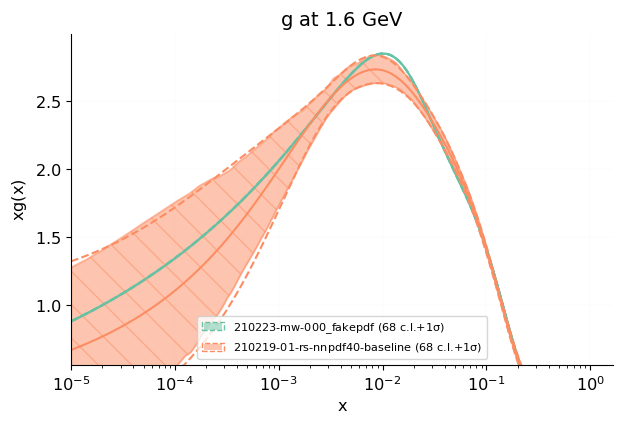
\includegraphics[width=0.6 \textwidth]{plot_pdfs_g.png}
    \caption{The green line is the input underlying law for the gluon PDF,
    which is sampled from the ensemble from a fit to data. The 68\% confidence
    interval is plotted for those replicas as the orange band.}
    \label{fig:InputGluonPDF}
\end{figure}


The observables used in the fits are a subset of the full NNPDF4.0 dataset.
For convenience,
we chose to fit the PDFs on a variant of the NNPDF3.1 dataset used in
\cite{Ball_2018}, which is described in detail in a study of the determination
of the strange PDF \cite{Faura_2020}. The datasets used in the calculation of
statistical estimators are the new datasets which will be included in NNPDF4.0,
and are summarised in Tab.~\ref{tab:summarise_new_data}, but not discussed in detail.

\begin{table}[h!]
    \begin{tabular}{lrrll}
\toprule
{} &  Training fraction &  Weight & C-factors &         Other fields \\
Dataset                                     &                    &         &           &                      \\
\midrule
DYE906R\_dw\_ite                              &               0.75 &       1 &  ACC, QCD &  custom\_group: unset \\
ATLASWZRAP11CF                              &               0.75 &       1 &       QCD &  custom\_group: unset \\
ATLASDY2D8TEV                               &               0.75 &       1 &    QCDEWK &  custom\_group: unset \\
ATLAS\_DY\_2D\_8TEV\_LOWMASS                    &               1.00 &       1 &       QCD &  custom\_group: unset \\
ATLAS\_WZ\_TOT\_13TEV                          &               1.00 &       1 &  NRM, QCD &  custom\_group: unset \\
ATLAS\_WP\_JET\_8TEV\_PT                        &               0.75 &       1 &       QCD &  custom\_group: unset \\
ATLAS\_WM\_JET\_8TEV\_PT                        &               0.75 &       1 &       QCD &  custom\_group: unset \\
ATLAS\_TTBARTOT\_13TEV\_FULLLUMI               &               0.75 &       1 &       QCD &  custom\_group: unset \\
ATLAS\_TTB\_DIFF\_8TEV\_LJ\_TTRAPNORM            &               1.00 &       1 &       QCD &  custom\_group: unset \\
ATLAS\_TOPDIFF\_DILEPT\_8TEV\_TTRAPNORM         &               1.00 &       1 &       QCD &  custom\_group: unset \\
ATLAS\_1JET\_8TEV\_R06\_DEC                     &               0.75 &       1 &       QCD &  custom\_group: unset \\
ATLAS\_2JET\_7TEV\_R06                         &               0.75 &       1 &       QCD &  custom\_group: unset \\
ATLASPHT15\_SF                               &               0.75 &       1 &  QCD, EWK &  custom\_group: unset \\
ATLAS\_SINGLETOP\_TCH\_R\_7TEV                  &               1.00 &       1 &       QCD &  custom\_group: unset \\
ATLAS\_SINGLETOP\_TCH\_R\_13TEV                 &               1.00 &       1 &       QCD &  custom\_group: unset \\
ATLAS\_SINGLETOP\_TCH\_DIFF\_7TEV\_T\_RAP\_NORM    &               1.00 &       1 &       QCD &  custom\_group: unset \\
ATLAS\_SINGLETOP\_TCH\_DIFF\_7TEV\_TBAR\_RAP\_NORM &               1.00 &       1 &       QCD &  custom\_group: unset \\
ATLAS\_SINGLETOP\_TCH\_DIFF\_8TEV\_T\_RAP\_NORM    &               0.75 &       1 &       QCD &  custom\_group: unset \\
ATLAS\_SINGLETOP\_TCH\_DIFF\_8TEV\_TBAR\_RAP\_NORM &               0.75 &       1 &       QCD &  custom\_group: unset \\
CMS\_2JET\_7TEV                               &               0.75 &       1 &       QCD &  custom\_group: unset \\
CMS\_2JET\_3D\_8TEV                            &               0.75 &       1 &       QCD &  custom\_group: unset \\
CMSTTBARTOT5TEV                             &               1.00 &       1 &       QCD &  custom\_group: unset \\
CMS\_TTBAR\_2D\_DIFF\_MTT\_TRAP\_NORM             &               1.00 &       1 &       QCD &  custom\_group: unset \\
CMS\_TTB\_DIFF\_13TEV\_2016\_2L\_TRAP             &               1.00 &       1 &       QCD &  custom\_group: unset \\
CMS\_TTB\_DIFF\_13TEV\_2016\_LJ\_TRAP             &               1.00 &       1 &       QCD &  custom\_group: unset \\
CMS\_SINGLETOP\_TCH\_TOT\_7TEV                  &               1.00 &       1 &       QCD &  custom\_group: unset \\
CMS\_SINGLETOP\_TCH\_R\_8TEV                    &               1.00 &       1 &       QCD &  custom\_group: unset \\
CMS\_SINGLETOP\_TCH\_R\_13TEV                   &               1.00 &       1 &       QCD &  custom\_group: unset \\
LHCB\_Z\_13TEV\_DIMUON                         &               1.00 &       1 &       QCD &  custom\_group: unset \\
LHCB\_Z\_13TEV\_DIELECTRON                     &               1.00 &       1 &       QCD &  custom\_group: unset \\
\bottomrule
\end{tabular}

    \caption{
        {\bf TODO: update to proper table with references.}
        Summary of datasets included in test set.
    }
    \label{tab:summarise_new_data}
\end{table}

The choice of fitted datasets is
considered unimportant, one could consider splitting the data into training
and test in a way which considered kinematic coverage rather than this
naive chronological splitting. Alternatively, since the data is generated from
the theory predictions produced by the input underlying law, one could even
produce completely artificial data using a different set of FK tables. From a
practical standpoint, using the NNPDF3.1 dataset and validating on the newly
included
datasets in 4.0 allowed us to validate the PDF uncertainities on data outside
of the kinematic coverage of data included in the fit. Furthermore, the data estimators
only give us local information on the PDF uncertainties and it seems
logical to split the data in this way since the results seem more applicable to
the reality of how the PDFs end up being used.

We then generate 30 different sets of experimental central values
(or L1 data), as discussed in Sec.~\ref{sec:closure-test-intro}, for the
fitted 3.1-like dataset.
Each set of experimental central values was then
fitted following NNPDF4.0 methodology \cite{NNPDF40},
producing 40 pseudo-data replicas.
\section{Numerical Setup and Results}

In this Section we first introduce the experimental setup used to run the
closure tests, and then discuss the actual results: following the study performed in 
Ref.~\cite{nnpdf30}, we first analyse the relative 
size of different component of PDFs uncertainties, comparing the changes between the old
and the new methodologies, used to produce the NNPDF3.1 and NNPDF4.0 sets of PDFs respectively; 
we then move to data space estimators, which have been computed only for NNPDF4.0
\footnote{comment about the fact that this is possible thanks to the fact that the code is now much faster}.
The results here act both as a proof of principle of new estimators presented in this paper but also
as part of a suite of methodological validation tools, see also the "future
tests" \cite{Cruz_Martinez_2021}, used to understand the PDF uncertainties of
the recent NNPDF4.0 set of PDFs. For the purpose of understanding how the
results here were produced, we will briefly describe the key features of the
NNPDF4.0 methodology, but refer the reader to NNPDF4.0 for a full discussion on
how these methodological choices were made, and the impact on performing PDF
fits to experimental data.

\subsection{Neural network parton distribution functions}

Using neural networks to fit PDFs has been discussed many times in previous
NNPDF publications, see for example \cite{nnpdf30, Ball_2017}. A new feature of
NNPDF4.0 will be that, for the default fit performed in the evolution basis, a
single neural network parameterises all 8 PDF flavours $\{ g, \Sigma, V, V_3,
V_8, T_3, T_8, T_{15} \}$ at the initial scale. The PDF for a single flavour $j$,
at the initial scale $Q_0 = 1.65~{\rm GeV}$ is given by
\begin{equation}
    f_j(x, Q_0) = NN(x, \ln x | \modelvec)_j * x^{1-\alpha_j} * (1-x)^{\beta_j},
\end{equation}
where $\alpha$ and $\beta$ are the preprocessing exponents, which control the
PDF behaviour at $x \to 0$ and $x \to 1$ respectively and $NN(x, \ln x |
\modelvec)_j$ is the $j^{\rm th}$ output of the neural network, which takes $x$
and $\ln x$ as input. As discussed in Sec.~\ref{sec:fit-reps}, an ensemble of
models is fitted, each one is an MAP estimator of the corresponding pseudo-data
it is fitted on. 
An optimization algorithm is used to try and find the parameters which maximise the likelihood.
In principle, the preprocessing exponents can also be varied during the fit
analogously to the neural network parameters, such as in \cite{Carrazza_2019},
or they can be randomly selected from a predetermined range as is done in
previous NNPDF releases, for example \cite{Ball_2017}. There are clearly many
choices with respect to hyperparameters, the discussion of how these choices
have been made is beyond the scope of this paper and left to the full NNPDF4.0
release \cite{NNPDF40}. A summary of the hyperparameters used to produce results
presented in this paper are provided in Tab.~\ref{tab:Hyperparams}.

%Something like the following should go in Sec 3, when defining the forward map for NNPDF
%Finally, the parton distributions themselves are not compared directly with
%data. Instead the observables quantities are obtained by performing convolutions
%with the PDFs, as discussed in \ref{eq:DISExample}. In practice the observables
%are obtained by convoluting the PDFs with FastKernel tables, presented in
%\cite{Ball_2010,Bertone_2017}, for each data point. The convolution depends on
%the process type of the observable, for DIS-like observables, such as in
%Eq.~\ref{eq:DISExample}, the convolution is performed with a single PDF. For
%hadronic observables the convolution is performed between two PDFs. 


\subsection{Closure test setup}

As input to the closure test, a single replica was drawn randomly from a
previous NNPDF fit to experimental data. We refer to this as the underlying law
and the corresponding predictions the true observable values. An example of the
gluon input is provided in Fig.~\ref{fig:InputGluonPDF}. In principle any
function could be used as underlying law, however it makes sense to use a
realistic input.

\begin{figure}
    \centering
    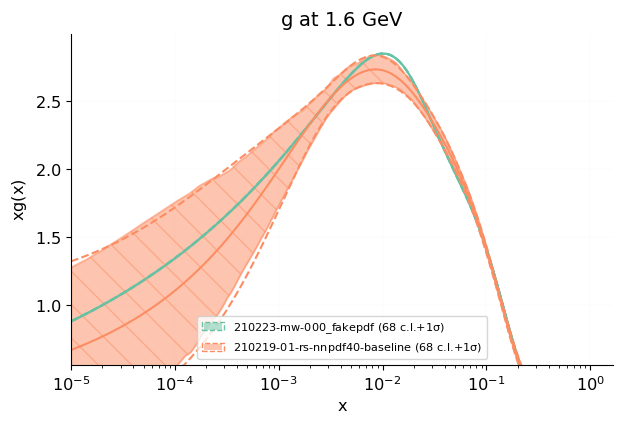
\includegraphics[width=0.8 \textwidth]{plot_pdfs_g.png}
    \caption{The green line is the input underlying law for the gluon PDF,
    which is sampled from the ensemble from a fit to data. The 68\% confidence
    interval is plotted for those replicas as the orange band.}
    \label{fig:InputGluonPDF}
\end{figure}

The observables used in the fits are a subset of the full NNPDF4.0 dataset. For
convenience, we chose to fit the PDFs on a variant of the NNPDF3.1 dataset used
in Ref.~\cite{Ball_2018}, which is described in detail in a study of the
determination of the strange PDF~\cite{Faura_2020}. The datasets used in the
calculation of statistical estimators are the new datasets which will be
included in NNPDF4.0, which will be discussed in detail with the main release.
For a full summary of observables used in the test data and a visual
representation of the kinematic region of both the training and testing data,
see App.~\ref{sec:appendix-datasets}.

The choice of data for both fitting and testing is considered unimportant, one
could consider splitting the data into training and test in a way which
considered kinematic coverage rather than this naive chronological splitting.
Alternatively, since the data is generated from the theory predictions produced
by the input underlying law, one could even produce completely artificial data
using a different set of FK tables. From a practical standpoint, using the
NNPDF3.1 dataset and validating on the newly included datasets in 4.0 allowed us
to validate the PDF uncertainities on data outside of the kinematic coverage of
data included in the fit. Furthermore, the data estimators only give us local
information on the PDF uncertainties and it seems logical to split the data in
this way since the results seem more applicable to the reality of how the PDFs
end up being used.

We then generate 30 different sets of experimental central values (or L1 data),
as discussed in Sec.~\ref{sec:closure-test-intro}, for the fitted 3.1-like
dataset. Each set of experimental central values was then fitted following
NNPDF4.0 methodology \cite{NNPDF40}, producing 40 pseudo-data replicas.

%When comparing with the old NNPDF methodology, we use the minimization algorithm
%of Ref.~\cite{nnpdf30}. An important iingredient of previous NNPDF minimization
%procedure was the choice of a stopping criterion. XXX

\subsection{Errors on PDFs}

As already discussed in Ref.~\cite{nnpdf30}, fitting to L0, L1 and L2
pseudo-data allows us to validate different aspects of the fitting procedure. In
an L0 fit, we fit multiple time the exact same set of data, which corresponds to
the theory prediction from the chosen model. The fitted pseudo-data is the
result obtained by applying the forward map to the model. It is clear that in
this case the quality of the fit can be improved at will, provided that the
parametrization is flexible enough and the minimization algorithm is efficient.
There are indeed multiple solutions that reproduce exactly the data set, while
interpolating between the data points. In an L1 the data have been fluctuated
around the theoretical prediction -- mimicking thereby the central values of
experimental measurements. The true model no longer reproduces the data; instead
it will yield a $\chi^2$ of order one. The pseudo-data are held fixed,
fluctuations from one replica to the next are due to the existence of multiple
solutions that hold a similar value for the residual $\chi^2$ at the end of the
minimization process. Finally, in the L2 fits, the fluctuations of the data are
reproduced by the replicas, and propagated to the model function when fitting
the data for each replica. Since the NNPDF fitting methodology has changed in
the latest release, it is important to compare the uncertainties at L0, L1 and
L2 that are obtained with the new fitting rouitne (n3fit) with the corresponding
ones obtained with the old fitting code (nnfit). 

An example of these relative errors on fitted PDFs is shown in Fig.~\ref{fig:CT_uncertainty_g}
for the case of the gluon distribution: L0, L1 and L2 closure tests are displayed on the same plot, each one
normalized to the corresponding central value. 
We note how the L0 and L1 uncertainties are the dominant ones in the $x$ regions where less experimental data are available,
namely at small and large-$x$, where the model is left unconstrained and free to fluctuate, while they are considerably
reduced in the data region. Here the L2 error, induced by the actual experimental data, is the dominant one.

It is interesting to compare these results with what we find with the old fitting code. The corresponding
plots are shown in Fig.~\ref{fig:CT_uncertainty_g_nnpdf3.1}: the PDF error 
is mainly dominated by the L0 uncertainty, even in those kinematic regions where experimental data are present.
This is in agreement with the results of Ref.~\cite{nnpdf30}, where it was shown that 
data uncertainties are not dominant anywhere.

This is clearly not the case for the results obtained with the new methodology.
This, most likely, is due to the different optimizers used in NNPDF4.0, which has been proved to be much more efficient 
than the genetic algorithm, adopted in the previous NNPDF determinations.

\begin{figure}[ht]
    \centering
    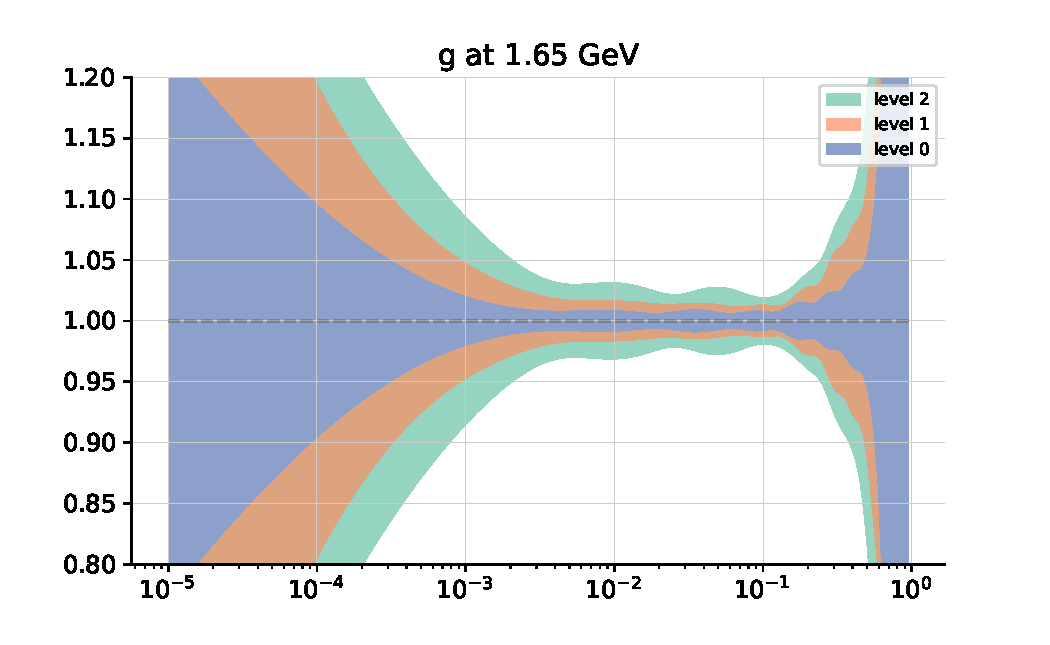
\includegraphics[scale=0.43]{CT_log_g.pdf}
    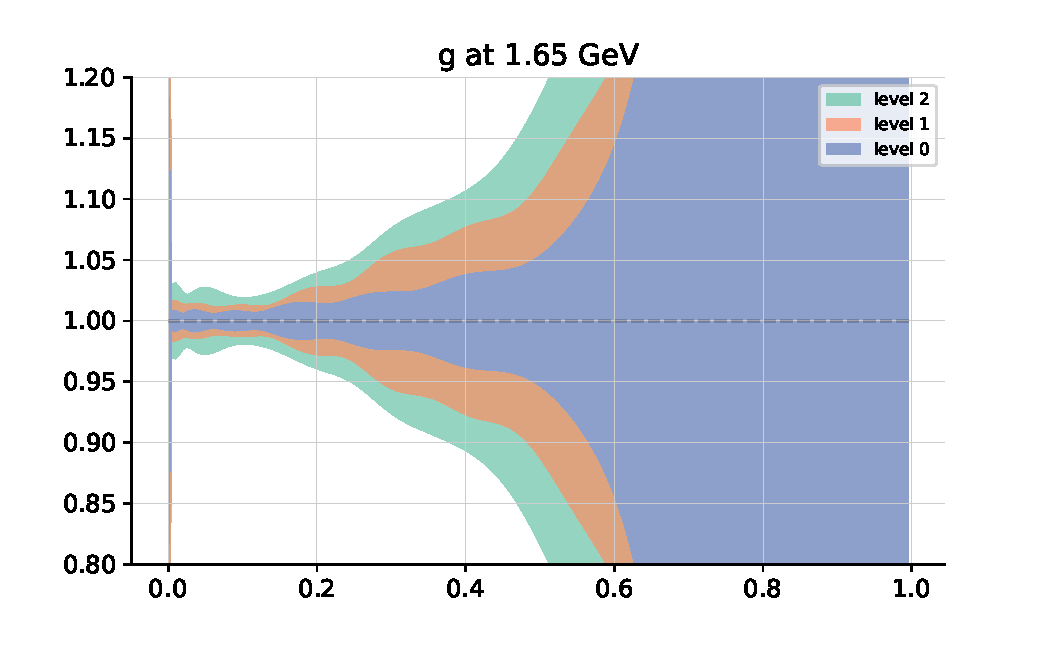
\includegraphics[scale=0.43]{CT_linear_g.pdf}
    \caption{Relative PDF error for the gluon distribution in the new methodology,
    plotted in logarithmic (left) and linear scale (right).}
    \label{fig:CT_uncertainty_g}    
\end{figure}

\begin{figure}[ht]
    \centering
    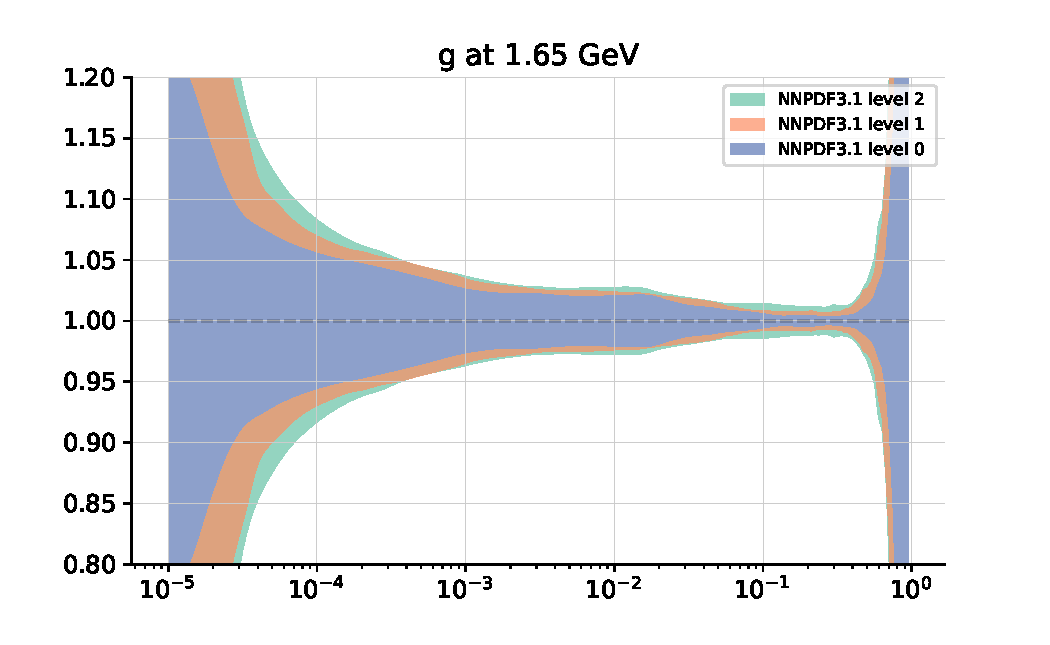
\includegraphics[scale=0.43]{CT_log_g_nnpdf31.pdf}
    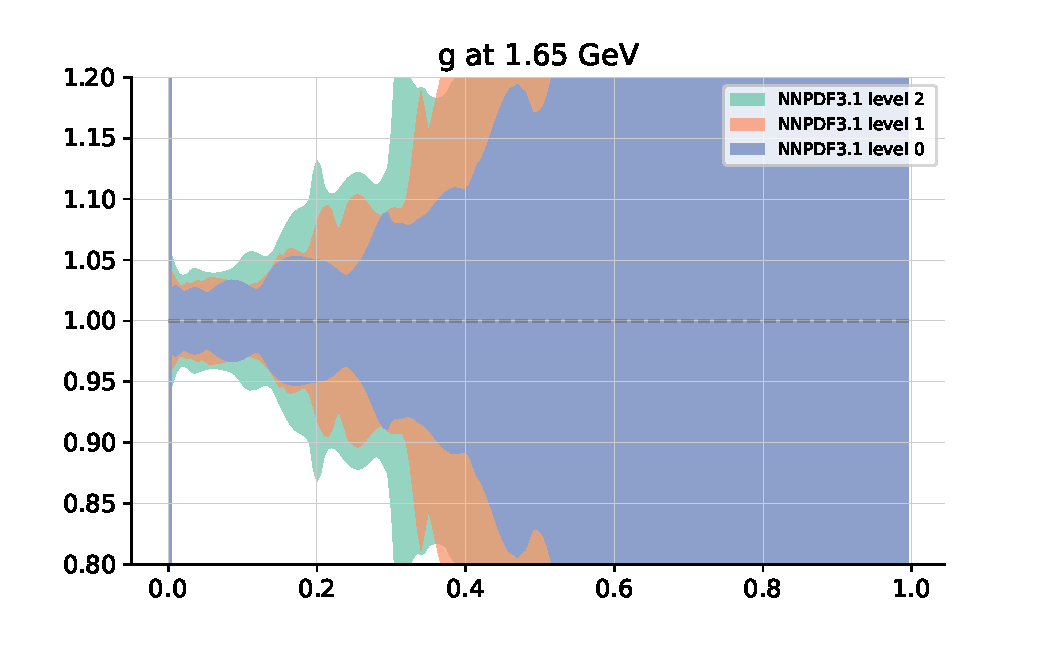
\includegraphics[scale=0.43]{CT_linear_g_nnpdf31.pdf}
    \caption{Same as Fig.~\ref{fig:CT_uncertainty_g} for the old methodology.}
    \label{fig:CT_uncertainty_g_nnpdf3.1}    
\end{figure}

%\begin{figure}[ht]
%    \centering
%    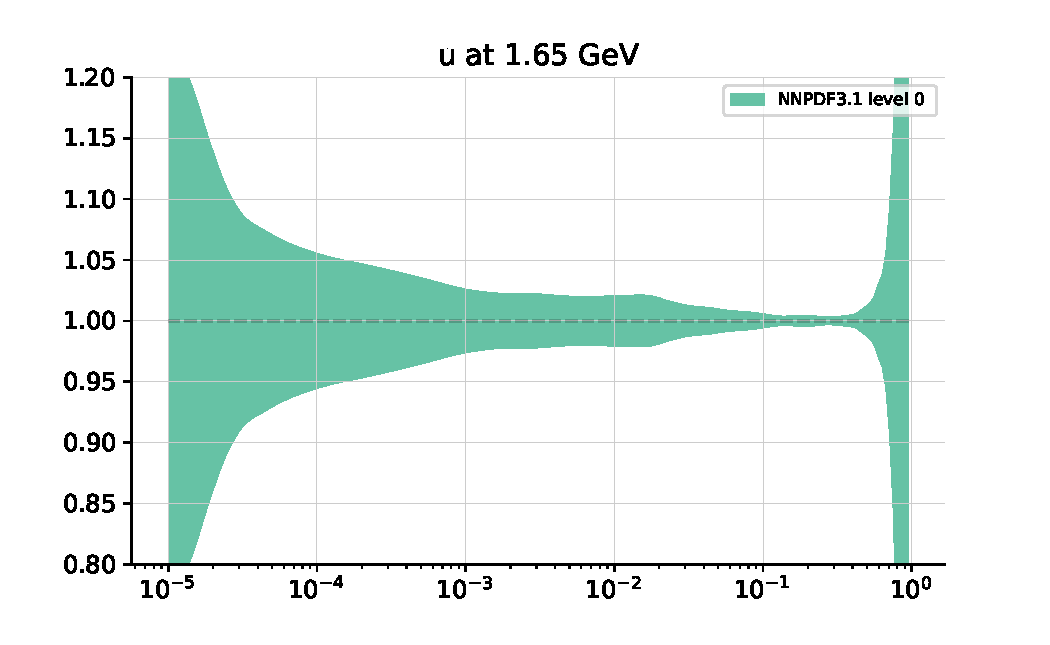
\includegraphics[scale=0.43]{CT_log_u_nnpdf31.pdf}
%    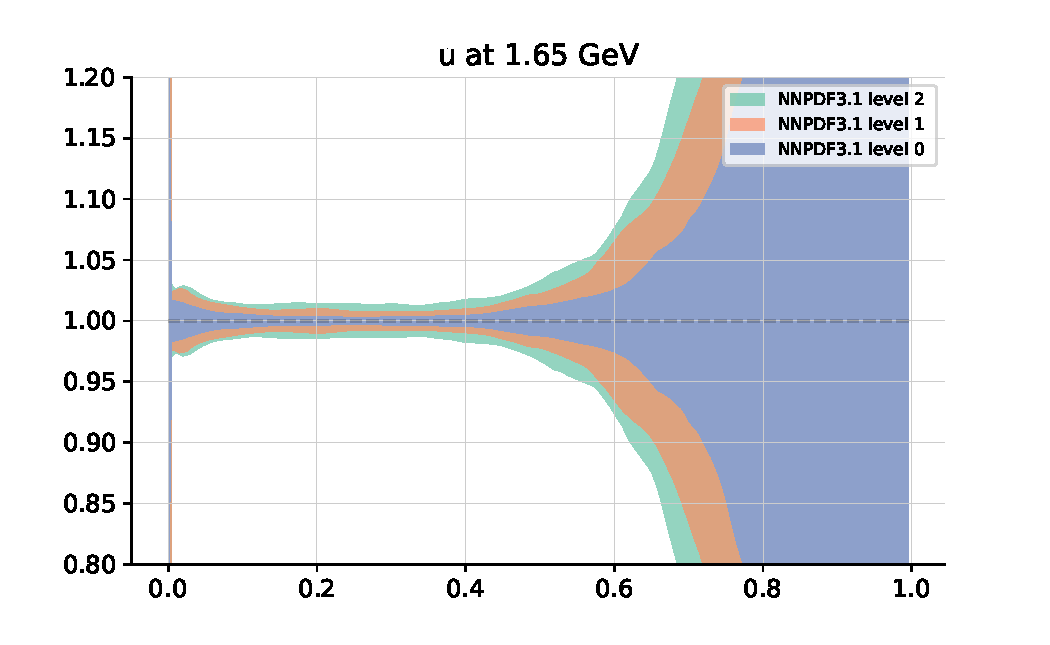
\includegraphics[scale=0.43]{CT_linear_u_nnpdf31.pdf}
%    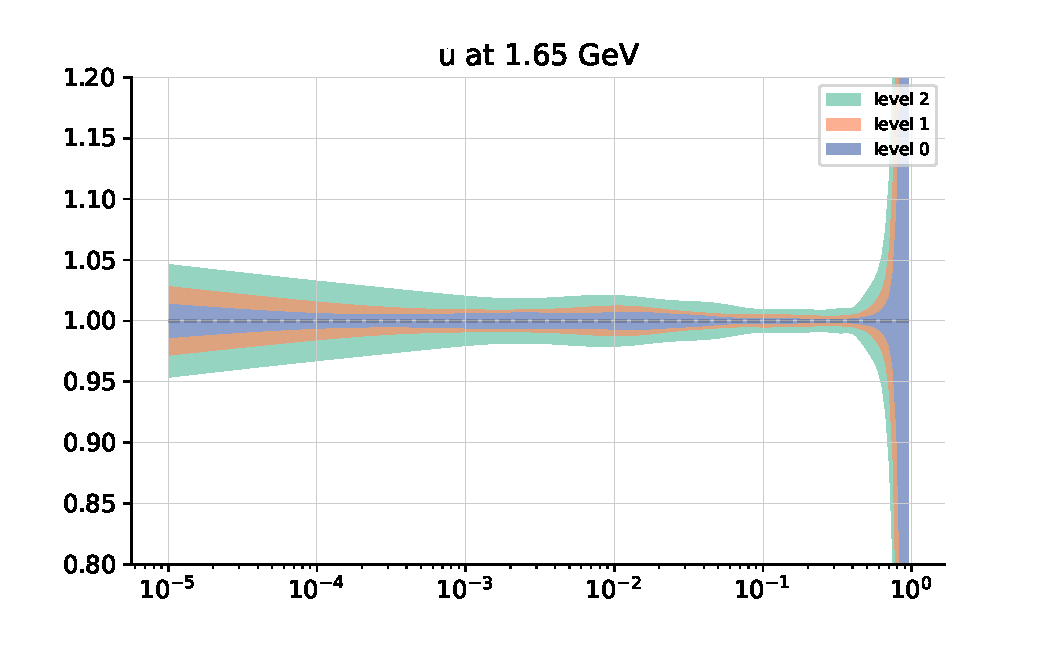
\includegraphics[scale=0.43]{CT_log_u.pdf}
%    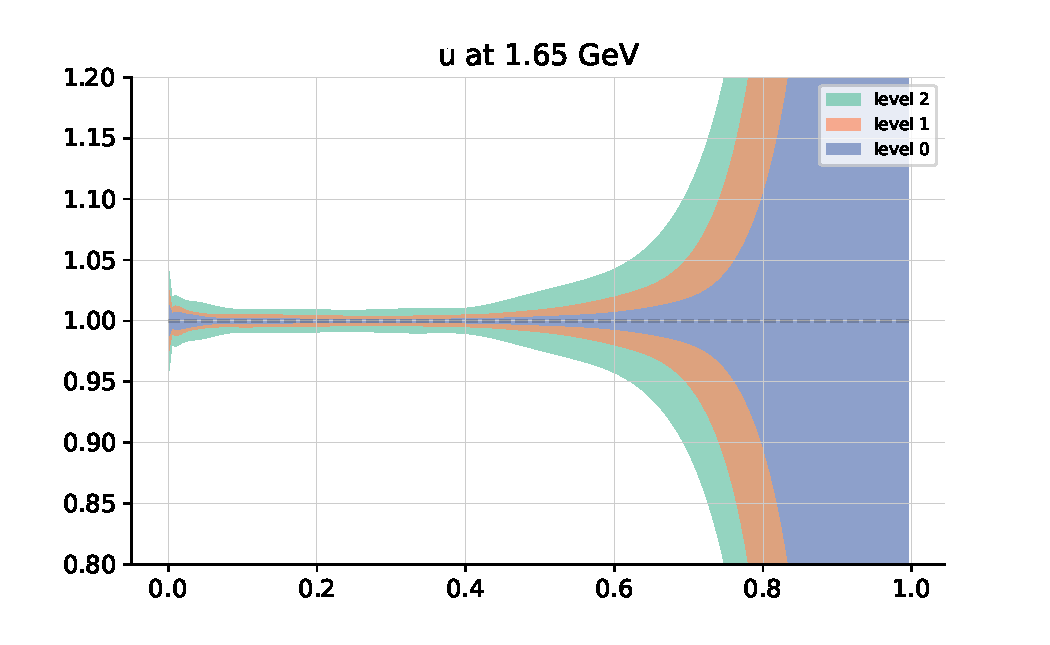
\includegraphics[scale=0.43]{CT_linear_u.pdf}
%    \caption{Same as Fig.~\ref{fig:CT_uncertainty_g} but for the up quark distribution.}
%    \label{fig:CT_uncertainty_u}    
%\end{figure}

\subsection{Bias-variance ratio}

We calculated $\biasvarratio$ on the test data, shown in
Tab.~\ref{tab:summarise_new_data}. An
uncertainty on $\biasvarratio$ by performing a bootstrap sample
\cite{efron1994introduction},
where we randomly sample from both fits and replicas and re-calculate
$\biasvarratio$, the value and error presented in the table is then the mean
and standard deviation across bootstrap samples. We checked that the distribution
of the estimator across bootstrap samples is indeed Gaussian. We also checked
that increasing the number of fits and replicas reduced the bootstrap error but
the central values were the same within the estimated bootstrap uncertainities.

\begin{table}[hb]
    \begin{center}
        \begin{tabular}{lr}
            \toprule
            {}     &  $\biasvarratio$ \\
            \midrule
            Total  &  $1.03\pm0.05$   \\
            \bottomrule
            \end{tabular}
    \end{center}
    \caption{
        The bias-variance ratio, $\biasvarratio$, for unseen data, summarised in
        Tab.~\ref{tab:summarise_new_data}. The uncertainty is estimated by
        performing a bootstrap sample across fits and replicas and calculating
        the standard deviation. We see that overall $\biasvarratio$ is consistent
        with 1, within uncertainities. This gives a good indication that, at least
        for the unseen data used in this study, the uncertainities are faithful.
    }
    \label{tab:biasvarratio}
\end{table}

One can also compare qualitatively the distribution of bias across fits, to the
distribution of the difference between replica predictions and expectation
values of predictions (in units of the covariance) across different fits
and replicas. The square root ratio of the mean of these two distributions
is precisely $\biasvarratio$.

\begin{figure}[ht]
    \centering
    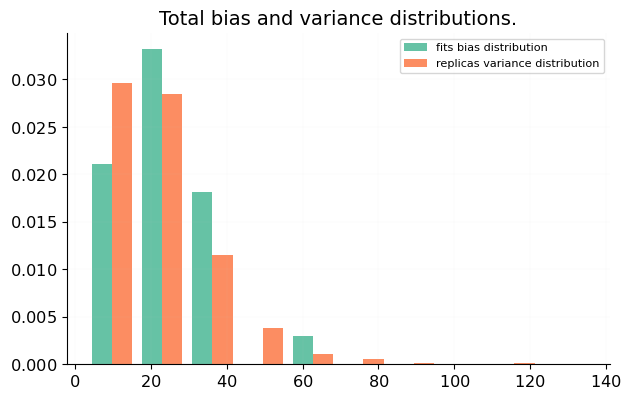
\includegraphics[width=0.8 \textwidth]{plot_bias_variance_distributions_total.png}
    \caption{The green histogram is the distribution of the total bias across fits,
    the orange histogram is the distribution of the difference between the
    replica and central predictions squared, in units of the covariance
    across all fits and replicas. This gives a qualitative picture of the full
    distribution, in Tab.~\ref{tab:biasvarratio} we compare the square root of the
    mean of each distribution.}
\end{figure}

\subsection{Comparison to quantile statistics}

As discussed in Sec.~\ref{sec:QuantileStatistics}, one can define an analogous
estimator in data space, based upon $\xi_{n\sigma}$, which was defined on a grid
of points in $x$ and $Q^2$ in PDF space in \cite{nnpdf30}. There is not
a one-to-one correspondence
between this and $\biasvarratio$, but a loose approximation using
Eq.~\ref{eq:expectedxi}. In Tab.~\ref{tab:xicomparison} we compare the estimated
$\xi_{1\sigma}$ from
subsituting $\biasvarratio$ into Eq.~\ref{eq:expectedxi} and to the
measured value.

\begin{table}[hb]
    \begin{center}
        \begin{tabular}{lrr}
            \toprule
            {}     & $\xi_{1\sigma}$ & $\erf(\biasvarratio/\sqrt{2})$ \\
            \midrule
            Total  & $0.69\pm0.02$   & $0.67\pm0.03$                  \\
            \bottomrule
            \end{tabular}
    \end{center}
    \caption{
        Comparing the measured value of $\xi_1\sigma$ and the estimated
        value from $\biasvarratio$. The two values are consistent, which
        suggests the approximation that the ratio of uncertainties is
        approximately the same across all data is not completely invalidated.
        Not only are the measured value and estimated value from $\biasvarratio$
        self consistent, but they are also consistent with $0.68$, which
        further supports the argument that the model uncertainities are
        faithful.
    }
    \label{tab:xicomparison}
\end{table}

Despite the assumptions entering each of the two estimators differing, we see
good agreement between the $\xi_{1\sigma}$ estimated from $\biasvarratio$
and that measured directly. We find this result reassuring, since it indicates
not only that the total uncertainty averaged across all data is faithful, but
also that the uncertainty on each data point seems faithful. If the results
differed it would indicate some kind of imbalance, where some components
of the uncertainty are correctly represented by the replicas but other directions
are not.

\section{Summary}

We've presented a formal framework for inverse problems, from a Bayesian
perspective. In particular, the framework provides a more formal description
of what it means when we talk about propagating experimental uncertainities
into the space of models. Strictly speaking, there is no fitting required to
obtain the expression for the posterior distributions in the space of the
data or the model, instead these are obtained by marginalising the
prior distribution. We note that sampling from the posterior distribution
of the model is,
in general, highly non-trivial but show that at least for linear problems the
NNPDF MC methodology can be shown to produce a sample of models which are
distributed according to the posterior model distribution. Furthermore, we
provide evidence that even for non-linear models this result at least holds
as a good approximation close to the MAP estimator.

We then use this formal framework to think about some of the estimators which
we use as part of the NNPDF closure test. In particular we derive bias and
variance from decomposing an out of sample error function, which is understood
from a classic fitting point of view.
The estimators are then related back to the posterior distributions in
the Bayesian framework. We note that the estimators themselves are not perfect
and suffer from only testing the model uncertainties locally (in regions where
the test data probes). Furthermore, the estimators only give an approximate
overall picture, and cannot be used to diagnose where the problem arises if
we find evidence that the model uncertaintes are not faithful.

Given the framework set out here, future work should be undertaken
generalise the closure estimators to model space. This would likely involve
a combination of the closure estimators presented here and 
the extension of the Bayesian framework to
infinite-dimensional spaces.

We give some preliminary closure results, as a proof of principle, the results
presented here will be examined in more detail alongside the full NNPDF4.0
release but serve as an example of how the data space estimators can be practically
included even in a rather complex setting. The NNPDF4.0 methodology
passes the closure test according to the estimators presented here,
providing evidence that for unseen data the current NNPDF methodology
appears to provide faithful uncertainities. The estimators are not limited to
this specific application, and the results presented demonstrate how
the data space estimators can be incorporated into any inverse problem.
As previously mentioned, a more
general set of estimators in model space would be the gold-standard and give
us confidence in our uncertainities for future observables which probe
regions which are not covered by either the training or testing data.

In the closure test framework described in this study, the prior on the
data is fully consistent with the generation of the 
observable central values from the true observables and uncertainities
by construction, which is likely not the case in real world fits. Something
which should be investigated is guarantee faithful uncertainities when this
is no longer the case, for example one could consider
a closure test where the generated data was inconsistent with the prior.
Most observed inconsistentency between the prior and the data
central values is likely due to missing theoretical uncertainities, but
once all sources of theoretical uncertainities have been accounted for
there could still be tension in the data. The advantage of viewing
inverse problems from a Bayesian perspective is access to
methodologies which deal with inconsistent data (or unknown
systematics) in a Bayesian framework,
for example in these cosmological studies \cite{Luis_Bernal_2018, Hobson_2002}.
These methods potentially offer a more formal approach to dealing with
inconsistent data, rather than ad hoc procedures.

The inclusion of MHOUs in the likelihood was justified from a Bayesian
perspective \cite{AbdulKhalek:2019ihb}, but here we have drawn a connection
between the model replicas and the posterior distribution in model space,
which explains why theoretical uncertainities
must be included in both the sampling of the pseudodata replicas and the
likelihood. Therefore we emphasise that the framework set out here is not
only useful for understanding model uncertainities with the current
methodology, but also for motivating future methodological development from
a Bayesian perspective.

% As a final thought, in light of the Bayesian framework set out here, one could
% even conceive of a methodology which
% used a different MC technique to sample directly from the posterior model
% distribution, for which we have an explicit (unnormalised) expression. This
% would be a complete paradigm shift from the approach described in
% Sec.~\ref{sec:fluct-fit-values} but could have some advantages, such as
% guaranteeing that the model replicas were exactly sampled from the posterior
% model distribution, even in the tails of the distribution far from the MAP
% estimator.

\appendix
\section{Gaussian integrals}
\label{sec:GaussianIntegrals}

Theory errors can be included in this framework by allowing the distribution of
observables around the theory prediction to have a finite width, \eg\ by
replacing the Dirac delta 
\begin{equation}
    \label{eq:DiracInApp}
    \delta(y-\mathcal{G}u)
\end{equation}
in Eq.~\ref{xxx} with a Gaussian 
\begin{equation}
    \label{eq:TheoryGaussian}
    \theta(\obs,\modelvec|\fwdobsop) \propto \exp\left[
        -\frac12 \left(y-\mathcal{G}u\right)^T
        C_T^{-1} \left(y-\mathcal{G}u\right)
    \right]\, .
\end{equation}
For the purposes of this study, we do not want to provide a realistic estimate
of theory errors. Instead we will be assuming that the errors are uncorrelated
and identical for all data points
\begin{equation}
    \label{eq:DiagTheoryCov}
    C_T = \sigma^2 \mathds{1}\, ,
\end{equation}
and we will be interested in the limit where $\sigma^2\to 0$. 

\subsection{Integrating out the data}
\label{sec:IntOutData}

Marginalizing with respect to \obs\ in this case yields 
\begin{align}
  \label{eq:MarginGaussData}
  \pi_M(\modelvec|\obspriorcent,\modelpriorcent,\fwdobsop) 
  &\propto \pi_{M}^0(\modelvec|\modelpriorcent) \, 
  \int dy\, \pi_{D}^0(\obs|\obspriorcent) 
    \theta(\obs,\modelvec|\fwdobsop) \, .
\end{align}
The argument of the exponential in the integrand is a quadratic form in \obs, 
\begin{equation}
    \label{eq:QuadFormDataInt}
    A = \left(y-y_0\right)^T C_D^{-1} \left(y-y_0\right) +
    \left(y-\mathcal{G}u\right)^T C_T^{-1} \left(y-\mathcal{G}u\right)\, .
\end{equation}
The integral can be easily evaluated by completing the square, 
\begin{equation}
    \label{eq:QuadFormDataIntSquare}
    A = \left(y-\tilde{y}\right)^T 
    \tilde{C}_D^{-1}
    \left(y-\tilde{y}\right) + R_D\, .
\end{equation}
Comparing Eqs.~\ref{eq:QuadFormDataInt} and~\ref{eq:QuadFormDataIntSquare} at order $y^2$ and \obs, yields
\begin{align}
    \tilde{C}_D^{-1} &= \frac{1}{\sigma^2}
    \left(\mathds{1} + \sigma^2 C_D^{-1}\right)\, , \\
    \tilde{y} &= \left(\mathds{1} + \sigma^2 C_D^{-1}\right)^{-1} 
    \left(
        \mathcal{G}u + \sigma^2 C_D^{-1} y_0
    \right)\, ,
\end{align}
and therefore
\begin{align}
    \tilde{y}^T \tilde{C}_D^{-1} \tilde{y}
    &= \frac{1}{\sigma^2} \left(\mathcal{G}u\right)^T
    \left(\mathds{1}+\sigma^2 C_D^{-1}\right)^{-1} \left(\mathcal{G}u\right) +
    y_0^T C_D^{-1} \left(\mathds{1}+\sigma^2 C_D^{-1}\right)^{-1} 
    \left(\mathcal{G}u\right) + \nonumber \\
    \label{eq:RemainderFromSquare}
    & \quad + \left(\mathcal{G}u\right)^T C_D^{-1} 
    \left(\mathds{1}+\sigma^2 C_D^{-1}\right)^{-1} y_0 + 
    \sigma^2 y_0^T C_D^{-1} \left(\mathds{1}+\sigma^2 C_D^{-1}\right)^{-1} 
    C_D^{-1} y_0\, .
\end{align}
Note that the four terms in the equation above are ordered in increasing powers
of $\sigma^2$ and ultimately we will be interested in the limit $\sigma^2\to 0$,
which reproduces the Dirac delta in $\theta(y,u)$. Plugging
Eq.~\ref{eq:RemainderFromSquare} in Eq.~\ref{eq:QuadFormDataIntSquare} and again
comparing to Eq.~\ref{eq:QuadFormDataInt}, we find
\begin{equation}
    \label{eq:RDBeforeLimit}  
    \begin{split}
    R_D 
    &= \frac{1}{\sigma^2} \left(\mathcal{G}u\right)^T 
    \left[
        \mathds{1} - \frac{1}{\mathds{1}+\sigma^2 C_D^{-1}} 
    \right]
    \left(\mathcal{G}u\right) - y_0^T C_D^{-1} \left(\mathcal{G}u\right)
    - \left(\mathcal{G}u\right)^T C_D^{-1} y_0 + \\ 
    & \quad + y_0^T C_D^{-1} y_0 + \mathcal{O}(\sigma^2)\, ,       
    \end{split} 
\end{equation}
Expanding for small values of $\sigma^2$ the terms of order $1/\sigma^2$ cancel;
keeping only finite terms in the limit $\sigma^2 \to 0$ we finally obtain
\begin{equation}
    \label{eq:RDAfterLimit}
    R_D = \left(\mathcal{G}u - y_0\right)^T C_D^{-1}
    \left(\mathcal{G}u - y_0\right)\, .
\end{equation}
This is exactly the result that we obtained earlier when 
\begin{equation}
    \label{eq:RemindTheta}
    \theta(y,u|\mathcal{G}) = \delta(y-\mathcal{G}u)\, .
\end{equation}
It should not come as a surprise since in the limit where $\sigma^2 \to 0$ the
Gaussian distribution that we chose to describe the fluctutations of the data
around the theory predictions reduces indeed to a Dirac delta. The posterior for
the model is exactly the one we computed in Sect.~\ref{sec:inverse-problems}. We
do not learn anything new from this exercise, but it is a useful warm-up for the
next example. The integral over \obs\ can now be performed easily, since it is
yet again a Gaussian integral. 


\subsection{Integrating out the model}
\label{eq:IntModOut}

Using the same approach as above, we now want to marginalise with respect to the model in order to obtain the posterior distribution of the data: 
\begin{align}
    \label{eq:MarginGaussModel}
    \pi_D(\obs|\obspriorcent,\modelpriorcent,\fwdobsop) 
    &\propto \pi_{D}^0(\obs|\obspriorcent) \, 
    \int du\, \pi_{M}^0(\modelvec|\modelpriorcent) 
      \theta(\obs,\modelvec|\fwdobsop) \, .
  \end{align}
We follow exactly the same procedure outlined above, starting from the argument
of the exponential
\begin{equation}
    \label{eq:QuadFormModelInt}
    A = \left(u-u_0\right)^T C_M^{-1} \left(u-u_0\right) +
    \left(y-\mathcal{G}u\right)^T C_T^{-1} \left(y-\mathcal{G}u\right)\, ,
\end{equation}
we complete the square and rewrite it in the form
\begin{equation}
    \label{eq:QuadFormModelIntSquare}
    A = \left(u-\tilde{u}\right)^T 
    \tilde{C}_M^{-1}
    \left(u-\tilde{u}\right) + R_M\, .
\end{equation}
It can be readily checked that in this case
\begin{align}
    \tilde{C}_M^{-1} &= \frac{1}{\sigma^2}
    \left(\mathcal{G}^T \mathcal{G} + \sigma^2 C_D^{-1}\right)\, , \\
    \tilde{u} &= \left(\mathcal{G}^T \mathcal{G} + \sigma^2 C_M^{-1}\right)
    \left(
        \mathcal{G}^T y + \sigma^2 C_M^{-1} u_0
    \right)\, .
\end{align}
In order to evaluate $R_M$, we need
\begin{equation}
    \label{eq:UtildeUtildeTerm}
    \begin{split}
    \tilde{u}^T \tilde{C}_M^{-1} \tilde{u} 
    &= \frac{1}{\sigma^2} y^T \mathcal{G} 
    \left(\mathcal{G}^T \mathcal{G} + \sigma^2 C_M^{-1}\right)^{-1}
    \mathcal{G}^T y +
    u_0^T C_M^{-1} 
    \left(\mathcal{G}^T \mathcal{G} + \sigma^2 C_M^{-1}\right)^{-1}
    \mathcal{G}^T y + \\
    & \quad + y^T \mathcal{G} \left(\mathcal{G}^T \mathcal{G} + \sigma^2 C_M^{-1}\right)^{-1} C_M^{-1} u_0 + \mathcal{O}(\sigma^2)\, .
    \end{split} 
\end{equation}
Noting that
\begin{equation}
    \label{eq:InverseFromTarantola}
    \left(\mathcal{G}^T \mathcal{G} + \sigma^2 C_M^{-1}\right)^{-1} =
    \frac{1}{\sigma^2} C_M - 
    \frac{1}{\sigma^2} C_M \mathcal{G}^T 
    \left(\mathcal{G} \frac{1}{\sigma^2} C_M \mathcal{G}^T 
        + \mathds{1}\right)^{-1} \mathcal{G}
    \frac{1}{\sigma^2} C_M\, ,
\end{equation}
we have, in the limit where $\sigma^2 \to 0$
\begin{equation}
    \label{eq:QuadraticYTerm}
    \mathcal{G} \left(\mathcal{G}^T \mathcal{G} + \sigma^2 C_M^{-1}\right)^{-1} 
    \mathcal{G}^T = 
    \mathds{1} - \sigma^2 \left(\mathcal{G} C_M \mathcal{G}^T\right)^{-1} + 
    \mathcal{O}(\sigma^4)\, .
\end{equation}
Collecting all terms we find
\begin{equation}
    \label{eq:RMAfterLimit}
    R_M = \left(y - \mathcal{G} u_0\right)^T 
        \left(\mathcal{G} C_M \mathcal{G}^T\right)^{-1}
        \left(y- \mathcal{G} u_0\right)\, .
\end{equation}
Performing the Gaussian integral over $u$ in Eq.~\ref{eq:MarginGaussModel}, the
posterior distribution of the data is:
\begin{equation}
    \label{eq:PosteriorDataDistr}
    \pi_D^y(y) \propto 
    \exp\left[-\frac12 \left(y-y_0\right)^T C_D^{-1} \left(y - y_0\right)
    -\frac12 \left(y - \mathcal{G} u_0\right)^T 
    \left(\mathcal{G} C_M \mathcal{G}^T\right)^{-1}
    \left(y - \mathcal{G} u_0\right)
    \right]\, .
\end{equation}
\section{Closure test setup details}
\label{sec:appendix-datasets}

\subsection{Data}

The full list of datasets included in the test set are shown in
Tab.~\ref{tab:summarise_new_data}. The central values are not actually used
in the closure test, however we use the experimental uncertainities in
the calculation of both $\biasvarratio$ and $\xisigdat{1}$. The corresponding
predictions generated from the underlying law are used as the true
observable values. Neither of the data-space closure estimators rely on
the central values of the test datasets.

\begin{table}[h!]
    \begin{center}
        \begin{tabular}{lc}
    \toprule
    Data set
    & Ref.
    \\
    \midrule
    DY E906 $\sigma^d_{\rm DY}/\sigma^p_{\rm DY}$ (SeaQuest)
    & \cite{Dove_2021}
    \\
    \midrule
    ATLAS $W,Z$ 7 TeV ($\mathcal{L}=4.6$~fb$^{-1}$)
    & \cite{Aaboud:2016btc}
    \\
    ATLAS DY 2D 8 TeV
    & \cite{Aaboud:2017ffb}
    \\
    ATLAS high-mass DY 2D 8 TeV
    & \cite{Aad:2016zzw}
    \\
    ATLAS $\sigma_{W,Z}$ 13 TeV
    & \cite{Aad:2016naf}
    \\
    ATLAS $W^+$+jet 8 TeV
    & \cite{Aaboud:2017soa}
    \\
    ATLAS $\sigma_{tt}^{\rm tot}$ 13 TeV ($\mathcal{L} = \SI{139}{\per\femto\barn}$)
    & \cite{Aad:2020tmz}
    \\
    ATLAS $t\bar{t}$ lepton+jets 8 TeV
    & \cite{Aad:2015mbv}
    \\
    ATLAS $t\bar{t}$ dilepton 8 TeV
    & \cite{Aaboud:2016iot}
    \\
    ATLAS single-inclusive jets 8 TeV, R=0.6
    & \cite{Aaboud:2017dvo}
    \\
    ATLAS dijets 7 TeV, R=0.6
    & \cite{Aad:2013tea}
    \\
    ATLAS direct photon production 13 TeV
    & \cite{Aaboud:2017cbm}
    \\
    ATLAS single top $R_{t}$ 7, 8, 13 TeV
    & \cite{Aad:2014fwa,Aaboud:2016ymp,Aaboud:2017pdi}
    \\
    \midrule
    CMS dijets 7 TeV
    & \cite{Chatrchyan:2012bja}
    \\
    CMS 3D dijets 8 TeV
    & \cite{Sirunyan:2017skj}
    \\
    CMS $\sigma_{tt}^{\rm tot}$ 5 TeV
    & \cite{Sirunyan:2017ule}
    \\
    CMS $t\bar{t}$ 2D dilepton 8 TeV
    & \cite{Sirunyan:2017azo}
    \\
    CMS $t\bar{t}$ lepton+jet 13 TeV
    & \cite{Sirunyan:2018wem}
    \\
    CMS $t\bar{t}$ dilepton 13 TeV
    & \cite{Sirunyan:2018ucr}
    \\
    CMS single top $\sigma_{t}+\sigma_{\bar{t}}$ 7 TeV
    & \cite{Chatrchyan:2012ep}
    \\
    CMS single top $R_{t}$ 8, 13 TeV
    & \cite{Khachatryan:2014iya,Sirunyan:2016cdg}
    \\
    \midrule
    LHCb $Z\to \mu\mu, ee$ 13 TeV
    & \cite{Aaij:2016mgv}
    \\
    \bottomrule
\end{tabular}
    \end{center}
    \caption{
        Observables included in the test data. We wish to stress that the observable
        central values themselves are not used, however the experimental
        uncertainities are used in the definition of the closure estimators, and
        the corresponding predictions from either the underlying law or the
        closure fits.
    }
    \label{tab:summarise_new_data}
\end{table}

For completeness, in Fig.~\ref{fig:DataKinematicCoverage}
the kinematic coverage of the training datasets, which
as mentioned is the NNPDF3.1-like dataset used in \cite{Faura_2020}, and the
test datasets shown in Tab.~\ref{tab:summarise_new_data} is plotted.

\begin{figure}
    \centering
    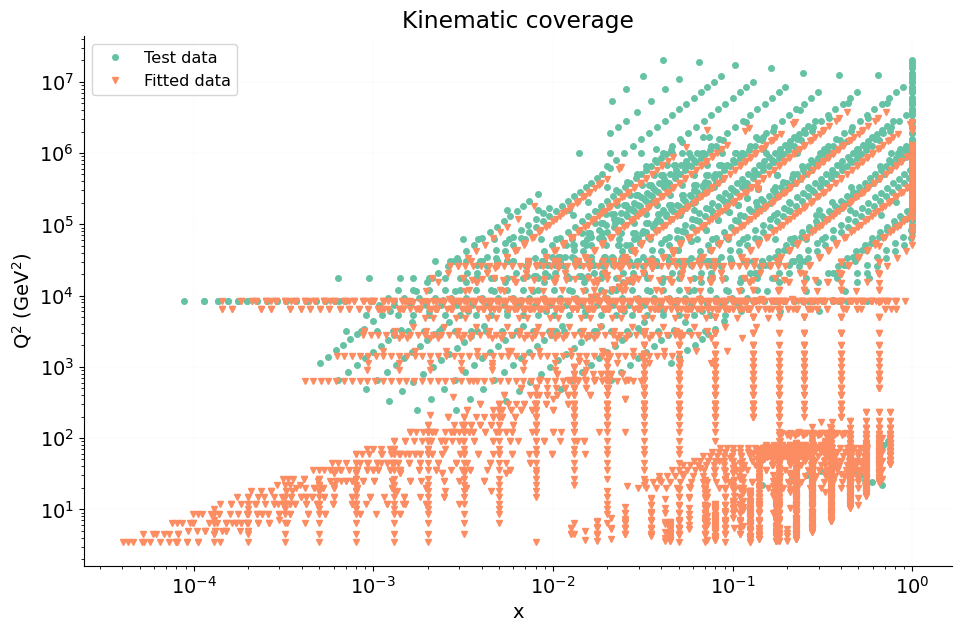
\includegraphics[width=0.8 \textwidth]{plot_xq2.png}
    % TODO: make PDF for higher res image.
    \caption{The kinematic coverage of the training and test data
    used to train the models and produce results presented in this paper. We emphasise
    that the split of datasets was largely chosen on practical grounds, not because
    of a deep reason to split the data chronologically. The kinematics of the two
    sets of data with this particular split overlaps but there are also kinematic
    regions which the test dataset probes, for which there was no training data.}
    \label{fig:DataKinematicCoverage}
\end{figure}

\subsection{Models}

A summary of the hyperparameters for the neural networks used during the closure
fits is given in table Tab.~\ref{tab:Hyperparams}. These hyperparameters were
chosen as part of an extensive hyperparameters scan, which will be explained in
detail in NNPDF4.0, for this study we simply provide the values of the
hyperparameters as a point of reference.

\begin{table}
    \begin{center}
        \begin{tabular}[h]{c|c}
            \toprule
            hyperparameter & value \\
            \midrule
            architecture & 2-25-20-8 \\
            activation & tanh-tanh-linear \\
            minimiser & NAdam \\
            max training length & 17000 epochs \\
            pre-processing exponents & not fitted \\
            \bottomrule
        \end{tabular}
    \end{center}
    \caption{Hyperparameters for neural networks used in this study. The parameter
    choices, and how these choices were made will be discussed in the full NNPDF4.0
    paper. The table here is simply to add context to the results below. There
    are 763 trainable parameters.}
    \label{tab:Hyperparams}
\end{table}
\section{Understanding NNPDF3.0 data estimators}

In the closure test presented in NNPDF3.0 \cite{nnpdf30} there was a data-space
estimator which aimed to measure the level of over or under fitting, $\deltachi$.
Here we discuss how $\deltachi$ can emerge from the bias-variance decomposition
and then use the linear model to try and understand it in the context of
viewing the ensemble of model replicas as a sample from the posterior distribution
of the model given the data.

Despite the link between the estimators emerging from the decomposition of
$\eout$ and the posterior distribution for data which is not used to inform
the model parameters, if we perform the same decomposition as in
Sec.~\ref{sec:ClosureEstimatorsDerivation} but set
$\testset{\obspriorcent}=\obspriorcent$ then we find that the cross term
in the final line of Eq.~\ref{eq:EoutDecomposition} does not go to zero when
the expectation across data is taken because there is a dependence on
$\obspriorcent$ in both the model predictions and the noisey data. As a result
we have to modify Eq.~\ref{eq:ExpectedBiasVariance} to be
\begin{equation}\label{eq:ExpectedBiasVarianceTraining}
    \mathbf{E}_{\obspriorcent}[\ein] =
    \mathbf{E}_{\obspriorcent}[\bias] + 
    \mathbf{E}_{\obspriorcent}[\var] +
    \mathbf{E}_{\obspriorcent}[{\rm noise}] +
    \mathbf{E}_{\obspriorcent}[\noisecross]\, ,
\end{equation}
where we refer now to the right hand side of
Eq.~\ref{eq:ExpectedBiasVarianceTraining} as $\ein$ because it's evaluated on the
data used to inform the model replicas.

Now we examine the definition of $\deltachi$ introduced
in~\cite{nnpdf30}, defined as the difference between the
$\chi^2$ between the expectation value of the model predictions and the level
one data, and the $\chi^2$ between the underlying observable values and the
level one data. In~\cite{nnpdf30} the denominator was also set to be the
second term in the numerator, however here we slightly re-define
$\deltachi$ to instead simply be normalised by the number of data points:
\begin{equation}\label{eq:deltachi2def1}
    \begin{split}
        \deltachi &= \\
            \frac{1}{\ndata} & \Big[ \left( \emodel{\fwdobsop\left(\modelvecrep\right)} - \obspriorcent \right)^T
            \obspriorcov^{-1}
            \left( \emodel{\fwdobsop\left(\modelvecrep\right)} - \obspriorcent \right) \\
            & \, - \left( \law - \obspriorcent \right)^T
            \obspriorcov^{-1}
            \left( \law - \obspriorcent \right)
        \Big] \\
        &= \bias + \noisecross \, ,
    \end{split}
\end{equation}
where in the second line we show how $\deltachi$ itself can be decomposed to
be equal to two of the terms in Eq.~\ref{eq:ExpectedBiasVarianceTraining}.

Constant values of $\deltachi$ define elliptical contours in data space
centered on the level one data. $\deltachi = 0$, in particular, defines a
contour which is centered on the level one data and passes through the
underlying law. When viewing $\deltachi$ from a classical fitting perspective,
if $\deltachi < 0$ then the expectation value of the model
predictions fit the level one data better than the underlying observables -
which indicates an overfitting of the shift, $\boldsymbol{\shift}$. Similarly,
$\deltachi > 0$ indicates some underfitting of the level one data.

If we return to the linear model we can write the analytic value of
$\deltachi$. Firstly, since $\testset{\obspriorcent}=\obspriorcent$ we can
simplify Eq.~\ref{eq:BiasLinearModel}
\begin{equation}\label{eq:BiasLinearModelSimple}
    \begin{split}
        \mathbf{E}_{\obspriorcent}[{\rm bias}] &= \frac{1}{\ndata}
            {\rm Tr} \left[
                \linmap \modelpostcov \linmap^T \obspriorcov^{-1}
            \right] \\
            &= \frac{1}{\ndata}{\rm Tr} \left[ \modelpostcov \modelpostcov^{-1}\right] \\
            &= \frac{\nmodel}{\ndata} \, ,
    \end{split}
\end{equation}
because $\modelpostcov \modelpostcov^{-1}$ is an $\nmodel \times \nmodel$ identity
matrix. Similarly we can write down the cross term
\begin{equation}
    \begin{split}
        \mathbf{E}_{\obspriorcent}[\noisecross] &= \frac{-2}{\ndata} \mathbf{E}_{\obspriorcent} \left[
            (\linmap \modelpostcov \linmap^T \obspriorcov^{-1} \obsnoise)^T \obspriorcov^{-1} \obsnoise
        \right] \\
        &= \frac{-2}{\ndata}{\rm Tr} [\linmap \modelpostcov \linmap^T \obspriorcov^{-1}] \\
        &= -2 \frac{\nmodel}{\ndata}
    \end{split}
\end{equation}
which leaves us with
\begin{equation}
    \mathbf{E}_{\obspriorcent}[\deltachi] = - \frac{\nmodel}{\ndata} \, .
\end{equation}
The point is that the linear model has already been shown to be a sample from
posterior distribution of the model given the data. But from the classical
fitting point of view we would say this model has overfitted.

As such, we do not report any results with $\deltachi$ here, because
when $\biasvarratio = 1$, it doesn't add much to the discussion. It may still
be useful as a diagnostic tool when $\biasvarratio \neq 1$, which as discussed
could be for a variety of reasons - including fitting inefficiency. It also
may be used as a performance indicator for deciding between two fitting
methodologies: if both fits are shown to have $\biasvarratio = 1$, the
methodology with smaller magnitude of $\deltachi$ could be preferential.
The same could be said for bias and variance however, bias in particular is
clearly closely related to $\deltachi$.

\bibliographystyle{unsrt}
\bibliography{biblio}

\end{document}

%%% Local Variables:
%%% mode: latex
%%% TeX-master: t
%%% End:
